% Options for packages loaded elsewhere
\PassOptionsToPackage{unicode}{hyperref}
\PassOptionsToPackage{hyphens}{url}
\PassOptionsToPackage{dvipsnames,svgnames,x11names}{xcolor}
%
\documentclass[
  letterpaper,
  DIV=11,
  numbers=noendperiod]{scrreprt}

\usepackage{amsmath,amssymb}
\usepackage{iftex}
\ifPDFTeX
  \usepackage[T1]{fontenc}
  \usepackage[utf8]{inputenc}
  \usepackage{textcomp} % provide euro and other symbols
\else % if luatex or xetex
  \usepackage{unicode-math}
  \defaultfontfeatures{Scale=MatchLowercase}
  \defaultfontfeatures[\rmfamily]{Ligatures=TeX,Scale=1}
\fi
\usepackage{lmodern}
\ifPDFTeX\else  
    % xetex/luatex font selection
\fi
% Use upquote if available, for straight quotes in verbatim environments
\IfFileExists{upquote.sty}{\usepackage{upquote}}{}
\IfFileExists{microtype.sty}{% use microtype if available
  \usepackage[]{microtype}
  \UseMicrotypeSet[protrusion]{basicmath} % disable protrusion for tt fonts
}{}
\makeatletter
\@ifundefined{KOMAClassName}{% if non-KOMA class
  \IfFileExists{parskip.sty}{%
    \usepackage{parskip}
  }{% else
    \setlength{\parindent}{0pt}
    \setlength{\parskip}{6pt plus 2pt minus 1pt}}
}{% if KOMA class
  \KOMAoptions{parskip=half}}
\makeatother
\usepackage{xcolor}
\setlength{\emergencystretch}{3em} % prevent overfull lines
\setcounter{secnumdepth}{5}
% Make \paragraph and \subparagraph free-standing
\makeatletter
\ifx\paragraph\undefined\else
  \let\oldparagraph\paragraph
  \renewcommand{\paragraph}{
    \@ifstar
      \xxxParagraphStar
      \xxxParagraphNoStar
  }
  \newcommand{\xxxParagraphStar}[1]{\oldparagraph*{#1}\mbox{}}
  \newcommand{\xxxParagraphNoStar}[1]{\oldparagraph{#1}\mbox{}}
\fi
\ifx\subparagraph\undefined\else
  \let\oldsubparagraph\subparagraph
  \renewcommand{\subparagraph}{
    \@ifstar
      \xxxSubParagraphStar
      \xxxSubParagraphNoStar
  }
  \newcommand{\xxxSubParagraphStar}[1]{\oldsubparagraph*{#1}\mbox{}}
  \newcommand{\xxxSubParagraphNoStar}[1]{\oldsubparagraph{#1}\mbox{}}
\fi
\makeatother


\providecommand{\tightlist}{%
  \setlength{\itemsep}{0pt}\setlength{\parskip}{0pt}}\usepackage{longtable,booktabs,array}
\usepackage{calc} % for calculating minipage widths
% Correct order of tables after \paragraph or \subparagraph
\usepackage{etoolbox}
\makeatletter
\patchcmd\longtable{\par}{\if@noskipsec\mbox{}\fi\par}{}{}
\makeatother
% Allow footnotes in longtable head/foot
\IfFileExists{footnotehyper.sty}{\usepackage{footnotehyper}}{\usepackage{footnote}}
\makesavenoteenv{longtable}
\usepackage{graphicx}
\makeatletter
\newsavebox\pandoc@box
\newcommand*\pandocbounded[1]{% scales image to fit in text height/width
  \sbox\pandoc@box{#1}%
  \Gscale@div\@tempa{\textheight}{\dimexpr\ht\pandoc@box+\dp\pandoc@box\relax}%
  \Gscale@div\@tempb{\linewidth}{\wd\pandoc@box}%
  \ifdim\@tempb\p@<\@tempa\p@\let\@tempa\@tempb\fi% select the smaller of both
  \ifdim\@tempa\p@<\p@\scalebox{\@tempa}{\usebox\pandoc@box}%
  \else\usebox{\pandoc@box}%
  \fi%
}
% Set default figure placement to htbp
\def\fps@figure{htbp}
\makeatother

\usepackage{cancel}
\KOMAoption{captions}{tableheading}
\makeatletter
\@ifpackageloaded{bookmark}{}{\usepackage{bookmark}}
\makeatother
\makeatletter
\@ifpackageloaded{caption}{}{\usepackage{caption}}
\AtBeginDocument{%
\ifdefined\contentsname
  \renewcommand*\contentsname{Table of contents}
\else
  \newcommand\contentsname{Table of contents}
\fi
\ifdefined\listfigurename
  \renewcommand*\listfigurename{List of Figures}
\else
  \newcommand\listfigurename{List of Figures}
\fi
\ifdefined\listtablename
  \renewcommand*\listtablename{List of Tables}
\else
  \newcommand\listtablename{List of Tables}
\fi
\ifdefined\figurename
  \renewcommand*\figurename{Figure}
\else
  \newcommand\figurename{Figure}
\fi
\ifdefined\tablename
  \renewcommand*\tablename{Table}
\else
  \newcommand\tablename{Table}
\fi
}
\@ifpackageloaded{float}{}{\usepackage{float}}
\floatstyle{ruled}
\@ifundefined{c@chapter}{\newfloat{codelisting}{h}{lop}}{\newfloat{codelisting}{h}{lop}[chapter]}
\floatname{codelisting}{Listing}
\newcommand*\listoflistings{\listof{codelisting}{List of Listings}}
\makeatother
\makeatletter
\makeatother
\makeatletter
\@ifpackageloaded{caption}{}{\usepackage{caption}}
\@ifpackageloaded{subcaption}{}{\usepackage{subcaption}}
\makeatother

\usepackage{bookmark}

\IfFileExists{xurl.sty}{\usepackage{xurl}}{} % add URL line breaks if available
\urlstyle{same} % disable monospaced font for URLs
\hypersetup{
  pdftitle={Physics 1 - Mechanics},
  pdfauthor={Yair Mau},
  colorlinks=true,
  linkcolor={blue},
  filecolor={Maroon},
  citecolor={Blue},
  urlcolor={Blue},
  pdfcreator={LaTeX via pandoc}}


\title{Physics 1 - Mechanics}
\author{Yair Mau}
\date{}

\begin{document}
\maketitle

\renewcommand*\contentsname{Table of contents}
{
\hypersetup{linkcolor=}
\setcounter{tocdepth}{2}
\tableofcontents
}

\bookmarksetup{startatroot}

\chapter*{about}\label{about}
\addcontentsline{toc}{chapter}{about}

\markboth{about}{about}

I taught the Physics 1 course in Mechanics at the Faculty of
Agriculture, Hebrew University, from 2017 to 2021. Although I don't
teach this any longer, I think that the materials I developed for the
course might be useful to some. Most of the material found here is in
hebrew.

\section*{goals}\label{goals}
\addcontentsline{toc}{section}{goals}

\markright{goals}

This basic Physics course has three main goals:

\begin{itemize}
\tightlist
\item
  By the end of this course you will be able to look at the world around
  you and start describing it in a formal (mathematical) language.
\item
  By the end of this course you will be able to read a graph and tell
  the story behind it, i.e., you will translate a formal (mathematical)
  language into regular speech any human can understand.
\item
  We will get acquainted with the concept of Energy. This, in my
  humblest opinion, is one of the most important ideas in Science.
\end{itemize}

\section*{patron saint}\label{patron-saint}
\addcontentsline{toc}{section}{patron saint}

\markright{patron saint}

Galileo is undoubtedly our hero in this course. Honorable runners-up:
Archimedes and Newton.

\pandocbounded{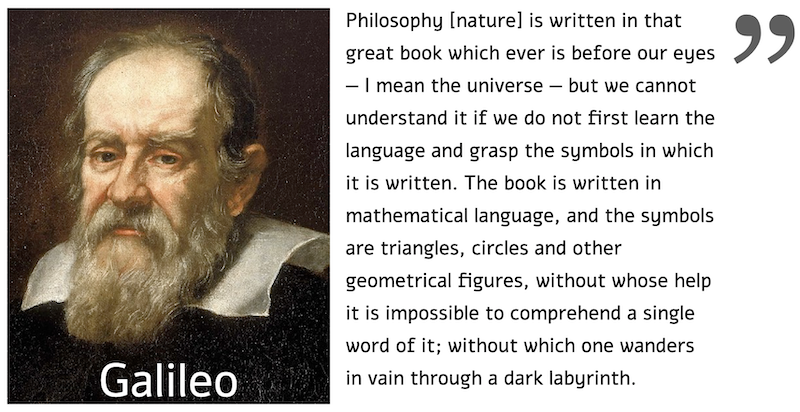
\includegraphics[keepaspectratio]{archive/gifs/Galileo-quote.png}}

\part{topics}

\chapter*{lecture notes}\label{lecture-notes}
\addcontentsline{toc}{chapter}{lecture notes}

\markboth{lecture notes}{lecture notes}

\textbf{Book:} I loosely use Halliday \& Resnick's \emph{Principles of
Physics} (11th edtion).\\
\textbf{Software:} I use \href{http://www.styluslabs.com/}{Stylus Labs
Write} to write my classnotes, it is available for Windows, Mac, Linux,
Android, and iOS.\\
\textbf{Hardware:} I use both a Wacom Cintiq 16 and an iPad air.\\
\textbf{Legend:}\\
lecture notes pdf\\
lecture notes source (write) svgz\\
powerpoint\\
widget in jupyter notebook (might take a while to load\ldots)\\
other materials\\
animations and gifs

\begin{longtable}[]{@{}
  >{\raggedright\arraybackslash}p{(\linewidth - 4\tabcolsep) * \real{0.3333}}
  >{\raggedright\arraybackslash}p{(\linewidth - 4\tabcolsep) * \real{0.3333}}
  >{\raggedright\arraybackslash}p{(\linewidth - 4\tabcolsep) * \real{0.3333}}@{}}
\toprule\noalign{}
\begin{minipage}[b]{\linewidth}\raggedright
subject
\end{minipage} & \begin{minipage}[b]{\linewidth}\raggedright
lectures
\end{minipage} & \begin{minipage}[b]{\linewidth}\raggedright
other
\end{minipage} \\
\midrule\noalign{}
\endhead
\bottomrule\noalign{}
\endlastfoot
basic math & & \href{./extra/extra-basic-math.qmd}{} \\
units & \href{./archive/lectures/guide-00-units.pdf}{}  
\href{./archive/lectures/guide-00-units.svgz}{} &
\href{extra/extra-units.qmd}{}   \href{./gifs/units.qmd}{} \\
1d kinematics & \href{./archive/lectures/guide-01-kinematics1d.pdf}{}  
\href{./archive/lectures/guide-01-kinematics1d.svgz}{} &
\href{./archive/lectures/kinematics1d.pptx}{}  
\href{https://mybinder.org/v2/gh/yairmau/website/HEAD?labpath=archive\%2Fphysics\%2Fwidgets\%2Finstantaneous_velocity.ipynb}{}
  \href{extra/extra-1d-kinematics.qmd}{}  
\href{./gifs/kinematics.qmd}{} \\
vectors & \href{./archive/lectures/guide-02-vectors.pdf}{}  
\href{./archive/lectures/guide-02-vectors.svgz}{} & \\
2d kinematics & \href{./archive/lectures/guide-02-kinematics-2d.pdf}{}  
\href{./archive/lectures/guide-kinematics-2d.svgz}{} &
\href{https://mybinder.org/v2/gh/yairmau/website/HEAD?labpath=archive\%2Fphysics\%2Fwidgets\%2Fmax_range_alpha.ipynb}{}
  \href{./gifs/kinematics.qmd}{} \\
circular motion &
\href{./archive/lectures/guide-02-circular-motion.pdf}{}  
\href{./archive/lectures/guide-02-circular-motion.svgz}{} &
\href{./archive/lectures/circular-motion.pptx}{}  
\href{./gifs/kinematics.qmd}{} \\
Newton's laws & \href{./archive/lectures/guide-03-newtons-laws.pdf}{}  
\href{./archive/lectures/guide-03-newtons-laws.svgz}{} &
\href{./archive/lectures/newton1and2.pptx}{}  
\href{./archive/lectures/newton3.pptx}{}  
\href{./gifs/newtons-laws.qmd}{} \\
work-energy theorem &
\href{./archive/lectures/guide-04-work-energy.pdf}{}  
\href{./archive/lectures/guide-04-work-energy.svgz}{} &
\href{https://mybinder.org/v2/gh/yairmau/website/HEAD?labpath=archive\%2Fphysics\%2Fwidgets\%2Friemann_integral.ipynb}{}
  \href{./gifs/energy.qmd}{} \\
potential energy &
\href{./archive/lectures/guide-04-potential-energy-U.pdf}{}  
\href{./archive/lectures/guide-04-potential-energy-U.svgz}{} &
\href{./gifs/energy.qmd}{} \\
potential energy diagrams &
\href{./archive/lectures/guide-04-potential-energy-diagram.pdf}{}  
\href{./archive/lectures/guide-04-potential-energy-diagram.svgz}{} & \\
linear momentum &
\href{./archive/lectures/guide-05-linear-momentum.pdf}{}  
\href{./archive/lectures/guide-05-linear-momentum.svgz}{} &
\href{./gifs/linear-momentum.qmd}{}  
\href{extra/extra-momentum.qmd}{} \\
gravitation & \href{./archive/lectures/guide-06-gravitation.pdf}{}  
\href{./archive/lectures/guide-06-gravitation.svgz}{} &
\href{./archive/lectures/earth-moon.pptx}{} \\
hydrostatics & \href{./archive/lectures/guide-07-hydrostatics.pdf}{}  
\href{./archive/lectures/guide-07-hydrostatics.svgz}{} &
\href{./gifs/fluids.qmd}{} \\
hydrodynamics & \href{./archive/lectures/guide-07-hydrodynamics.pdf}{}  
\href{./archive/lectures/guide-07-hydrodynamics.svgz}{} &
\href{./archive/lectures/hydrodynamics.pptx}{}  
\href{./gifs/fluids.qmd}{} \\
\end{longtable}

\href{https://docs.google.com/spreadsheets/d/1b0t98d7-tW82mCmukKrkjHK8gLdNHGRLrD-HxN_luNc/edit\#gid=0}{Click
here} for details on all lectures of the 2021-22 academic year.\\
Here are other \href{./gifs/wow.qmd}{very nice videos} not directly
related to any specific topic.

\chapter*{extra: basic math}\label{extra-basic-math}
\addcontentsline{toc}{chapter}{extra: basic math}

\markboth{extra: basic math}{extra: basic math}

I will assume that student in this course have a minimal proficiency in
math. Find below some links for basic math that we will need during this
course. I will not teach any of these topics, if you feel that you don't
fully know this stuff, please go ahead and study these topics asap.

\section*{Trigonometry}\label{trigonometry}
\addcontentsline{toc}{section}{Trigonometry}

\markright{Trigonometry}

\href{https://www.khanacademy.org/math/trigonometry}{Khan Academy}\\
\href{http://www.ilectureonline.com/lectures/subject/MATH/16}{Michel van
Biezen}

\section*{Pre-algebra}\label{pre-algebra}
\addcontentsline{toc}{section}{Pre-algebra}

\markright{Pre-algebra}

Arithmetic properties; factors and multiples; fractions; decimals;
negative numbers and coordinate plane; rations, rates, proportions;
equations, expressions, and inequalities; exponents, radicals, and
scientific notation.

\href{https://www.khanacademy.org/math/pre-algebra}{Khan Academy}

\section*{Algebra}\label{algebra}
\addcontentsline{toc}{section}{Algebra}

\markright{Algebra}

\href{http://www.ilectureonline.com/lectures/subject/MATH/14}{Michel van
Biezen}

\section*{עברית}\label{ux5e2ux5d1ux5e8ux5d9ux5ea}
\addcontentsline{toc}{section}{עברית}

\markright{עברית}

קיים אתר של אקדמיית קהאן בעברית, \href{http://www.hebrewkhan.org/}{כדאי
להכיר אותו}

\chapter*{extra: units}\label{extra-units}
\addcontentsline{toc}{chapter}{extra: units}

\markboth{extra: units}{extra: units}

\section*{basic units and prefixes}\label{basic-units-and-prefixes}
\addcontentsline{toc}{section}{basic units and prefixes}

\markright{basic units and prefixes}

Units for three SI base quantities

\begin{longtable}[]{@{}lll@{}}
\toprule\noalign{}
Quantity & Unit Name & Unit Symbol \\
\midrule\noalign{}
\endhead
\bottomrule\noalign{}
\endlastfoot
Length {[}L{]} & meter & m \\
Time {[}T{]} & second & s \\
Mass {[}M{]} & kilogram & kg \\
\end{longtable}

Some prefixes for SI Units that you \textbf{must} remember!

\begin{longtable}[]{@{}lll@{}}
\toprule\noalign{}
Factor & Prefix & Symbol \\
\midrule\noalign{}
\endhead
\bottomrule\noalign{}
\endlastfoot
\(10^9\) & giga- & G \\
\(10^6\) & mega- & M \\
\(10^3\) & kilo- & k \\
\(10^{-2}\) & centi- & c \\
\(10^{-3}\) & milli- & m \\
\(10^{-6}\) & micro- & \(\mu\) \\
\(10^{-9}\) & nano- & n \\
\end{longtable}

\section*{exponent rules}\label{exponent-rules}
\addcontentsline{toc}{section}{exponent rules}

\markright{exponent rules}

\pandocbounded{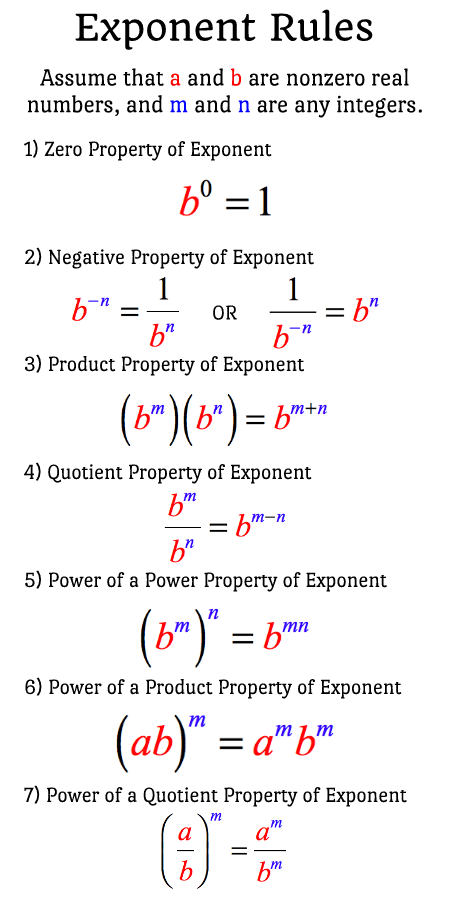
\includegraphics[keepaspectratio]{archive/gifs/exponents.png}}

\section*{volume and surface area}\label{volume-and-surface-area}
\addcontentsline{toc}{section}{volume and surface area}

\markright{volume and surface area}

\pandocbounded{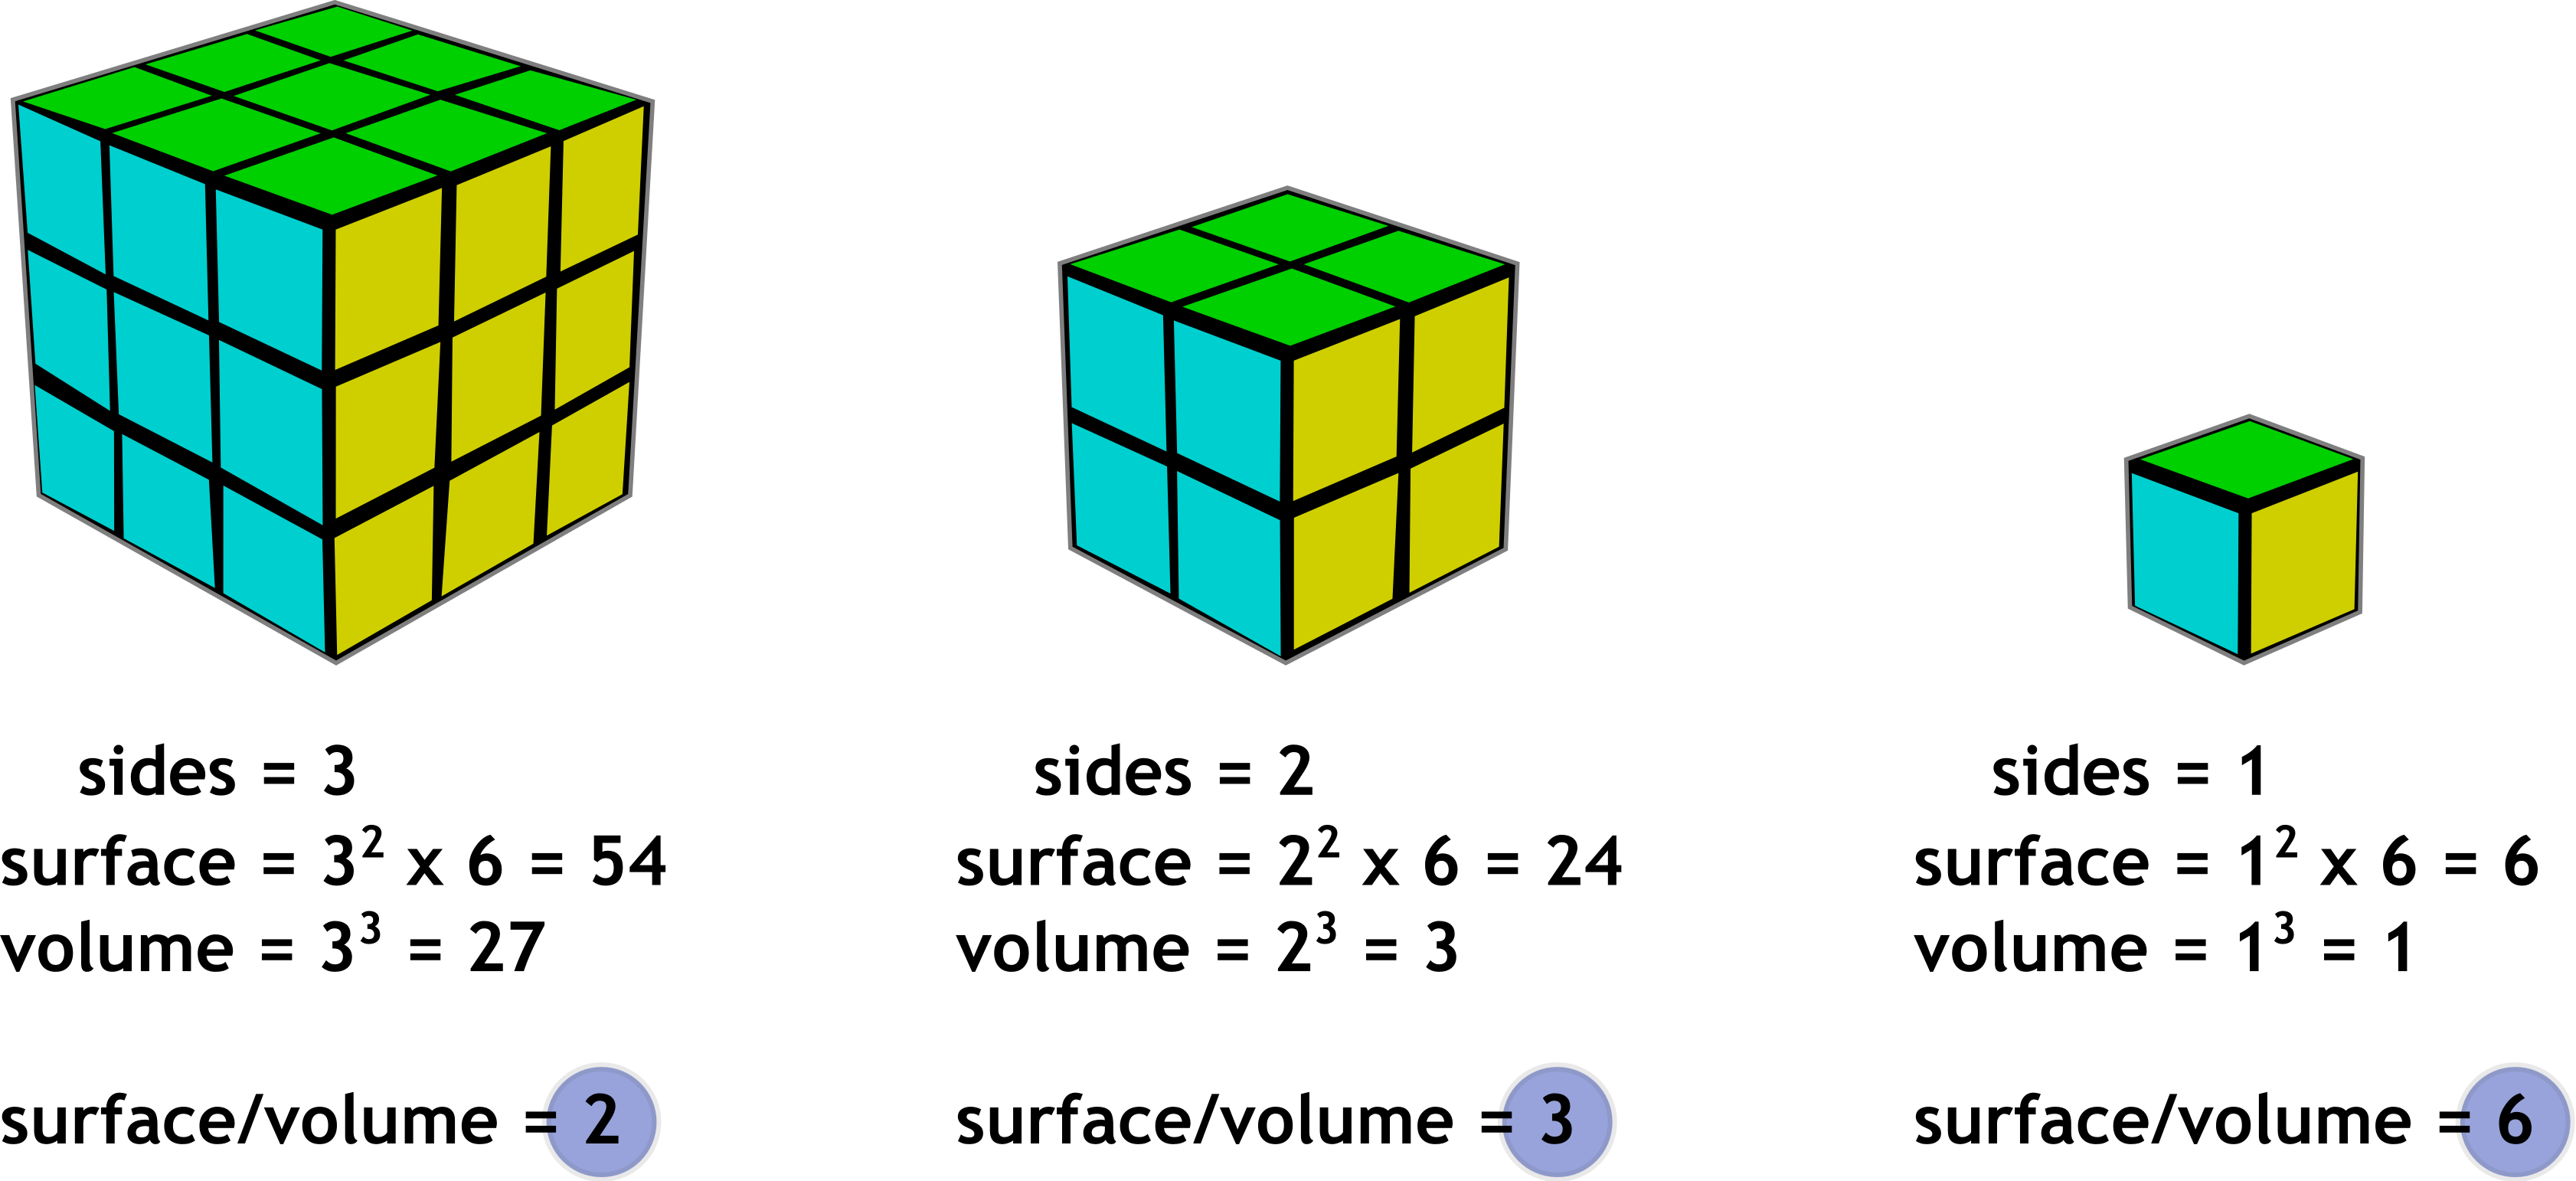
\includegraphics[keepaspectratio]{archive/gifs/surface_area_to_volume_ratio.png}}

\section*{1 horse-sized duck or 100 duck-sized
horses?}\label{horse-sized-duck-or-100-duck-sized-horses}
\addcontentsline{toc}{section}{1 horse-sized duck or 100 duck-sized
horses?}

\markright{1 horse-sized duck or 100 duck-sized horses?}

\pandocbounded{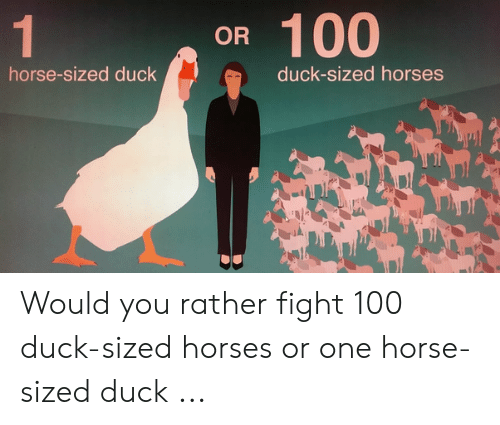
\includegraphics[keepaspectratio]{archive/gifs/duck-horse.png}}

\chapter*{extra: 1d kinematics}\label{extra-1d-kinematics}
\addcontentsline{toc}{chapter}{extra: 1d kinematics}

\markboth{extra: 1d kinematics}{extra: 1d kinematics}

\section*{The Physics Classroom}\label{the-physics-classroom}
\addcontentsline{toc}{section}{The Physics Classroom}

\markright{The Physics Classroom}

This is an \emph{excellent} interactive website, with lots of useful
exercises:\\
\href{http://www.physicsclassroom.com/Concept-Builders/Kinematics/Distance-vs-Displacement/Interactive}{Distance
vs.~Displacement}, \url{Acceleration},
\href{http://www.physicsclassroom.com/Concept-Builders/Kinematics/Name-That-Motion/Concept-Builder}{Name
That Motion},
\href{http://www.physicsclassroom.com/Concept-Builders/Kinematics/Motion-Diagrams/Interactive}{Motion
Diagrams},
\href{http://www.physicsclassroom.com/Concept-Builders/Kinematics/Graph-That-Motion/Concept-Builder}{Graph
That Motion}, \href{Match\%20That\%20Graph}{Match That Graph},
\href{http://www.physicsclassroom.com/Concept-Builders/Kinematics/Position-Time-Graphs-Conceptual-Analysis/Concept-Builder}{Position-Time
Graphs - Conceptual Analysis},
\href{http://www.physicsclassroom.com/Concept-Builders/Kinematics/Position-Time-Graphs/Concept-Builder}{Position-Time
Graphs - Numerical Analysis},
\href{http://www.physicsclassroom.com/Concept-Builders/Kinematics/Dots-And-Graphs/Concept-Builder}{Dots
and Graphs},
\href{http://www.physicsclassroom.com/Concept-Builders/Kinematics/Which-One-Doesnt-Belong/Concept-Builder}{Which
One Doesn't Belong?},
\href{http://www.physicsclassroom.com/Concept-Builders/Kinematics/Free-Fall/Concept-Builder}{Free
Fall},
\href{http://www.physicsclassroom.com/Concept-Builders/Kinematics/Up-and-Down/Concept-Builder}{Up
and Down}.

\section*{Video Lectures}\label{video-lectures}
\addcontentsline{toc}{section}{Video Lectures}

\markright{Video Lectures}

\href{https://www.khanacademy.org/science/physics/one-dimensional-motion}{Khan
Academy - One-dimensional motion}\\
\href{https://www.youtube.com/watch?v=ZM8ECpBuQYE}{Motion in a Straight
Line: Crash Course Physics \#1}\\
\href{http://www.ilectureonline.com/lectures/subject/PHYSICS/1/9}{Michel
van Biezen - Lectures in MOTION IN ONE DIMENSION}\\
\href{http://www.ilectureonline.com/lectures/subject/PHYSICS/1/230}{Michel
van Biezen - Lectures in Motion in 1 Dimension: GRAPHIC SOLUTIONS}

\section*{\texorpdfstring{\(x\), \(v\), \(a\)
graphs}{x, v, a graphs}}\label{x-v-a-graphs}
\addcontentsline{toc}{section}{\(x\), \(v\), \(a\) graphs}

\markright{\(x\), \(v\), \(a\) graphs}

Draw the missing curves, with black dots in the same instants in time as
in the given curve. All curved lines are parabolas.

\textbf{Exercise 1}
\pandocbounded{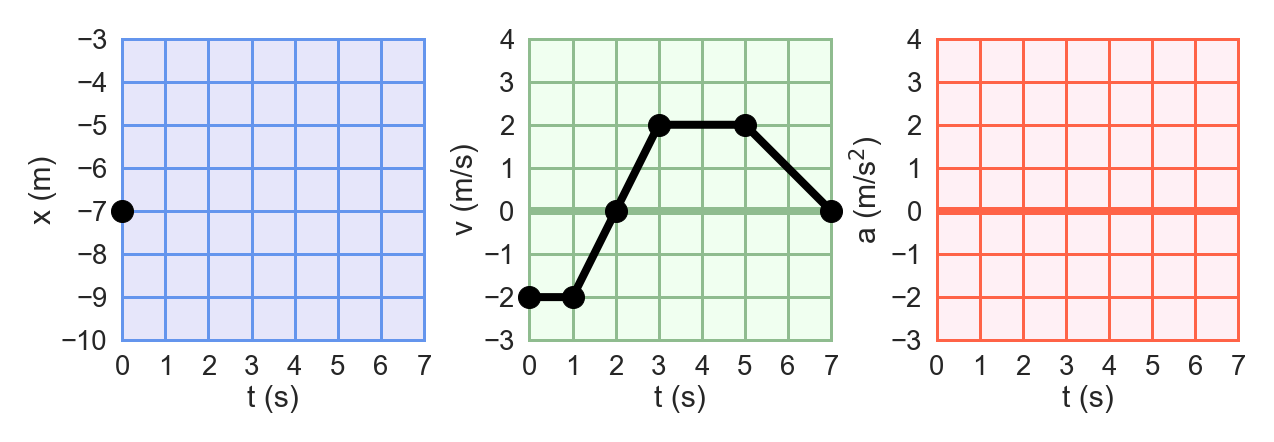
\includegraphics[keepaspectratio]{archive/gifs/3graphs_001_ques.png}}

\textbf{Exercise 2}
\pandocbounded{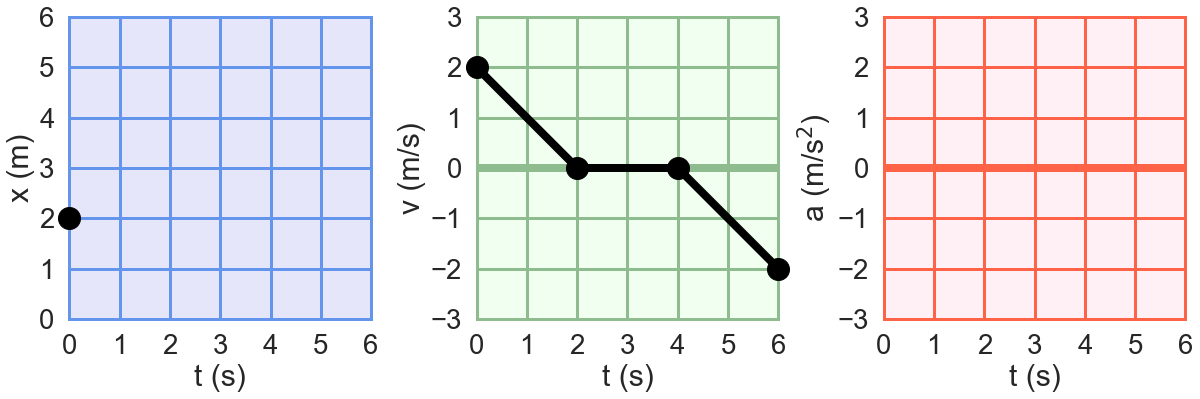
\includegraphics[keepaspectratio]{archive/gifs/3graphs_002_ques.png}}
\href{./archive/gifs/3graphs_002_answ.png}{}

\textbf{Exercise 3}
\pandocbounded{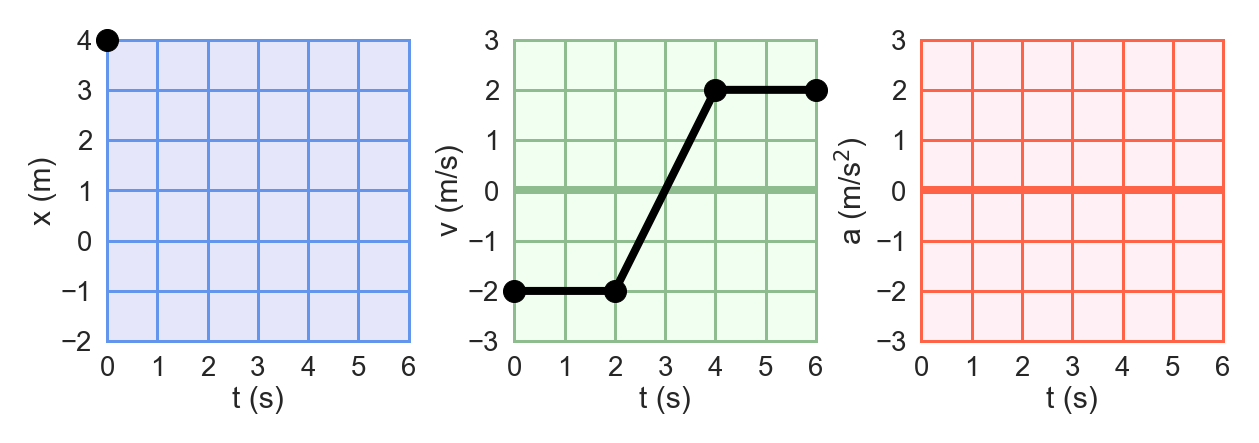
\includegraphics[keepaspectratio]{archive/gifs/3graphs_003_ques.png}}
\href{./archive/gifs/3graphs_003_answ.png}{}

\textbf{Exercise 4}
\pandocbounded{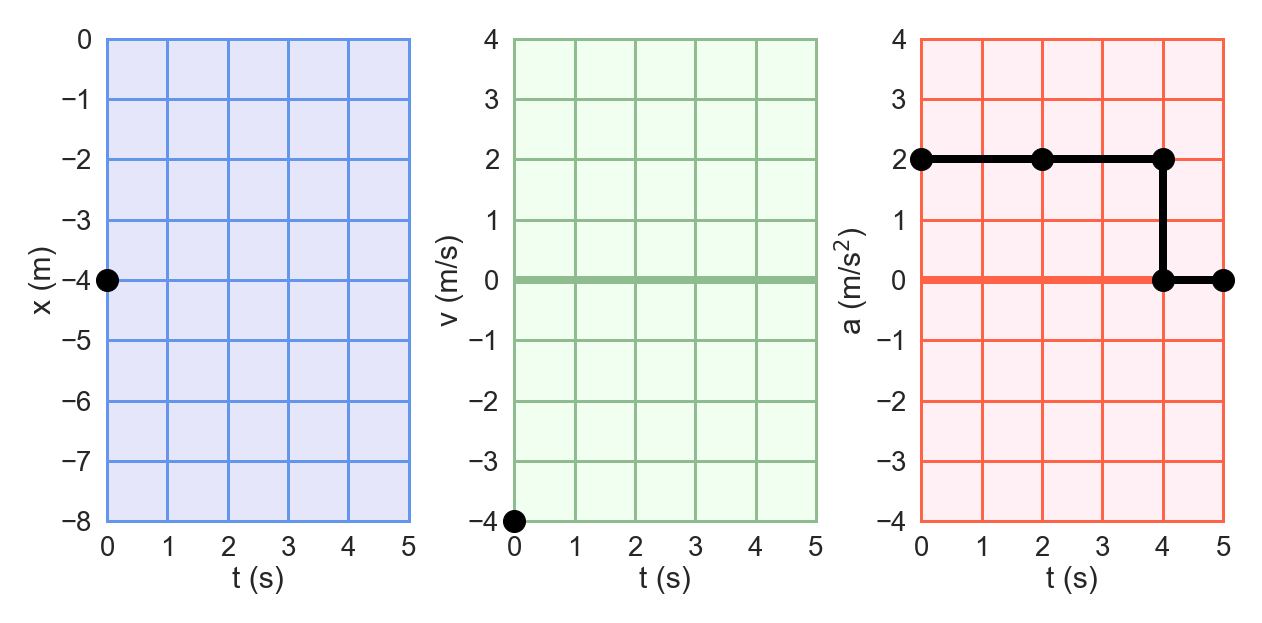
\includegraphics[keepaspectratio]{archive/gifs/3graphs_004_ques.png}}
\href{./archive/gifs/3graphs_004_answ.png}{}

\textbf{Exercise 5}
\pandocbounded{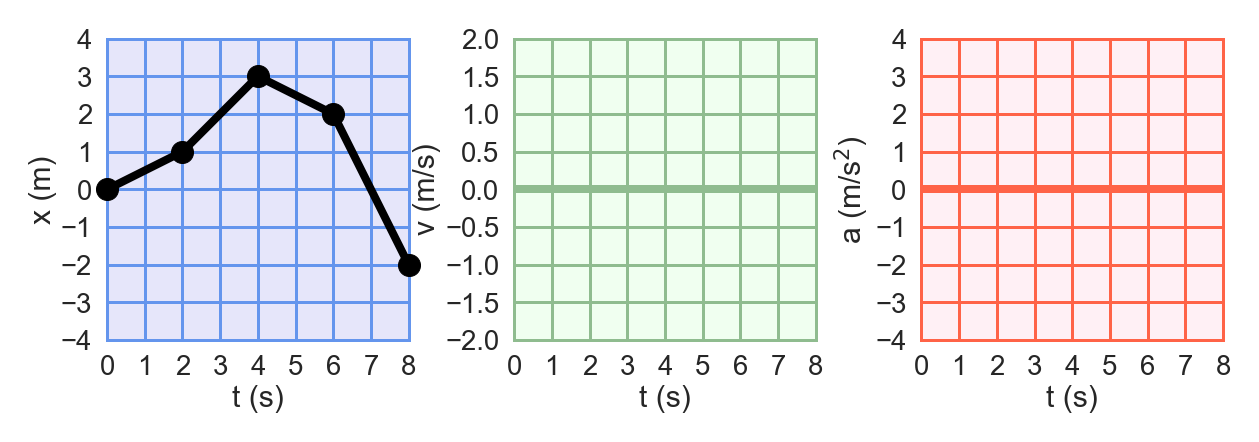
\includegraphics[keepaspectratio]{archive/gifs/3graphs_005_ques.png}}
\href{./archive/gifs/3graphs_005_answ.png}{}

\textbf{Exercise 6}
\pandocbounded{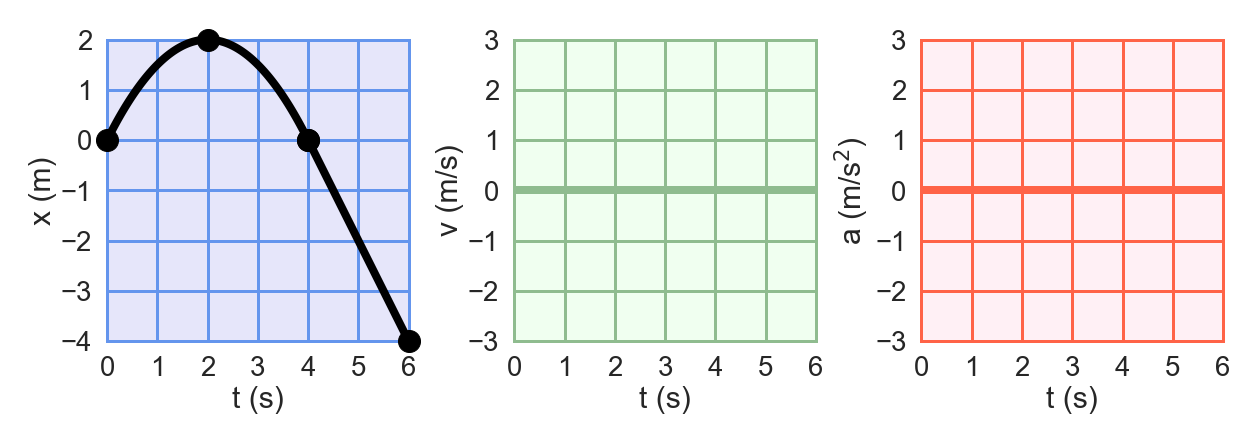
\includegraphics[keepaspectratio]{archive/gifs/3graphs_006_ques.png}}
\href{./archive/gifs/3graphs_006_answ.png}{}

\section*{\texorpdfstring{Match the graphs, \(x\) and
\(v\)}{Match the graphs, x and v}}\label{match-the-graphs-x-and-v}
\addcontentsline{toc}{section}{Match the graphs, \(x\) and \(v\)}

\markright{Match the graphs, \(x\) and \(v\)}

Match the curve on the left with one of the curves on the right.

\textbf{Exercise 1}
\pandocbounded{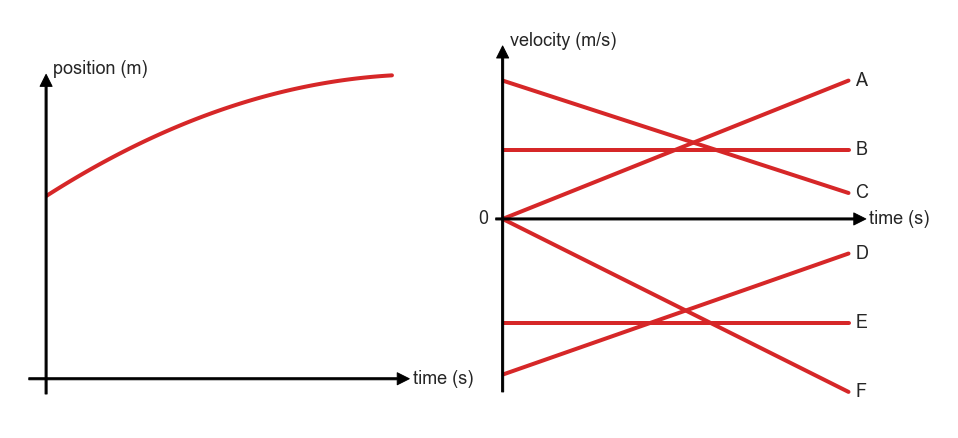
\includegraphics[keepaspectratio]{archive/gifs/match_x_v_001.png}}

\textbf{Exercise 2}
\pandocbounded{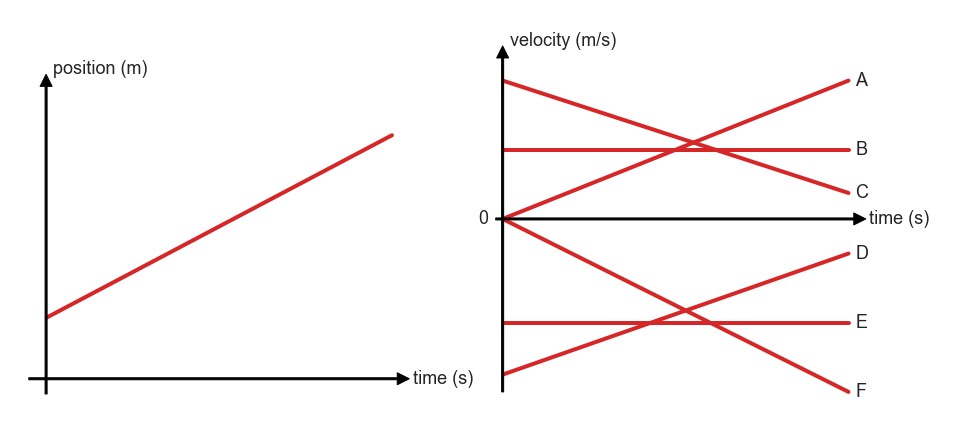
\includegraphics[keepaspectratio]{archive/gifs/match_x_v_002.png}}

\textbf{Exercise 3}
\pandocbounded{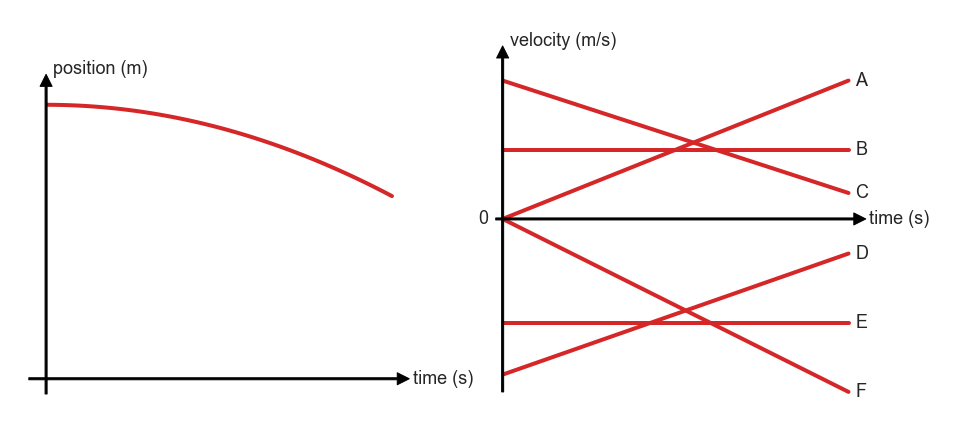
\includegraphics[keepaspectratio]{archive/gifs/match_x_v_003.png}}

\textbf{Exercise 4}
\pandocbounded{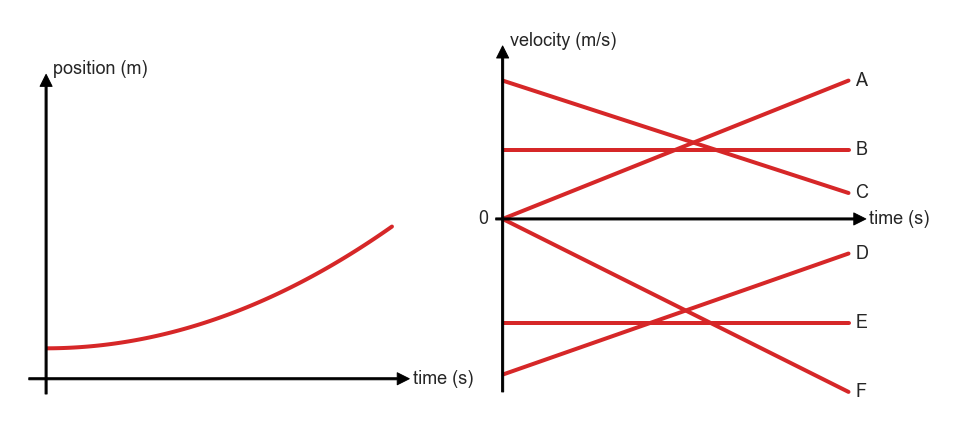
\includegraphics[keepaspectratio]{archive/gifs/match_x_v_004.png}}

\textbf{Exercise 5}
\pandocbounded{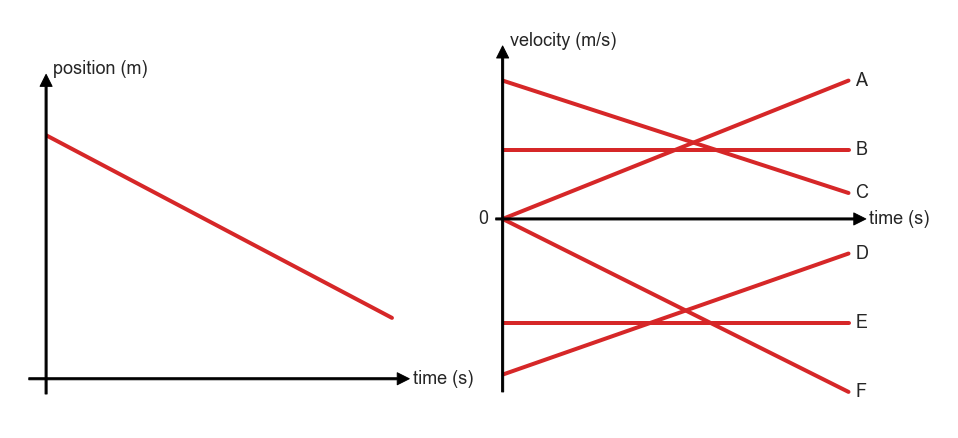
\includegraphics[keepaspectratio]{archive/gifs/match_x_v_005.png}}

\textbf{Exercise 6}
\pandocbounded{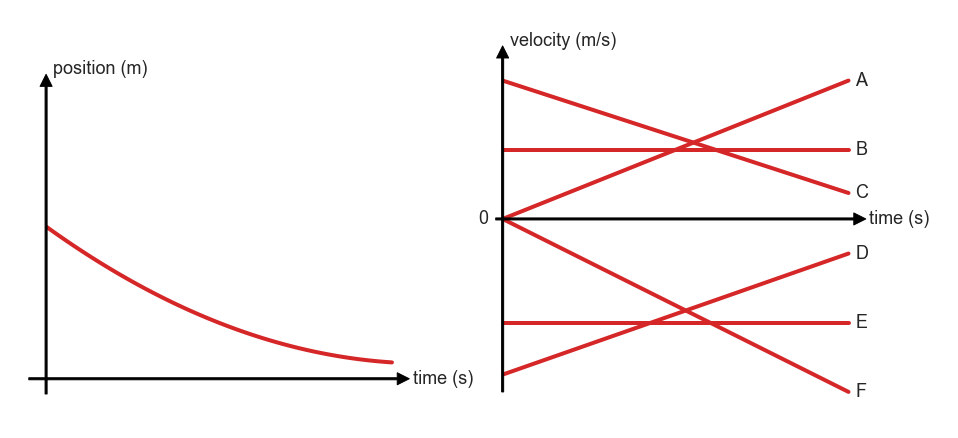
\includegraphics[keepaspectratio]{archive/gifs/match_x_v_006.png}}

\textbf{Exercise 7}
\pandocbounded{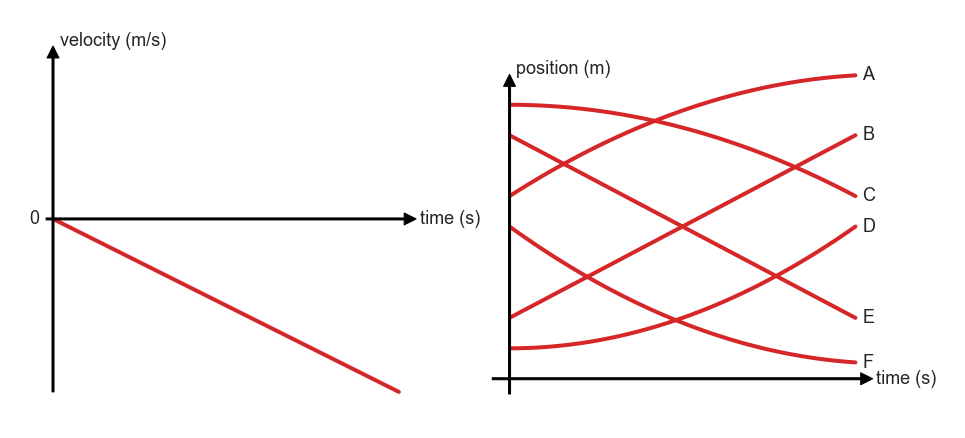
\includegraphics[keepaspectratio]{archive/gifs/match_x_v_007.png}}

\textbf{Exercise 8}
\pandocbounded{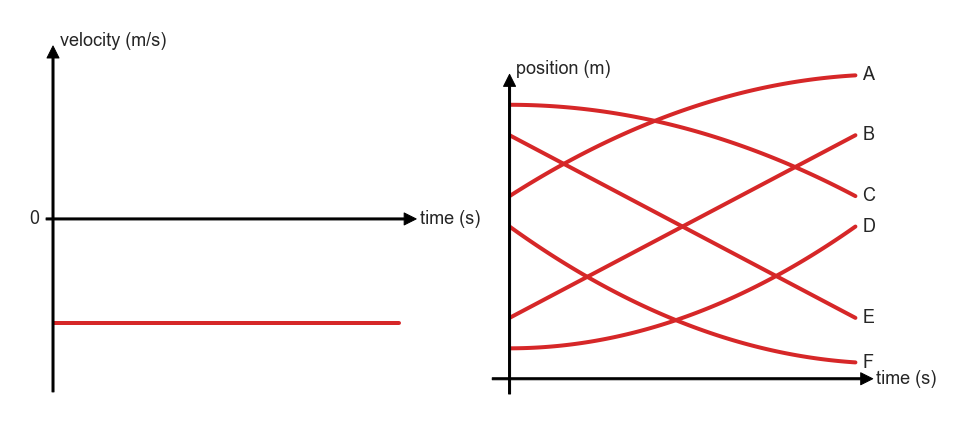
\includegraphics[keepaspectratio]{archive/gifs/match_x_v_008.png}}

\textbf{Exercise 9}
\pandocbounded{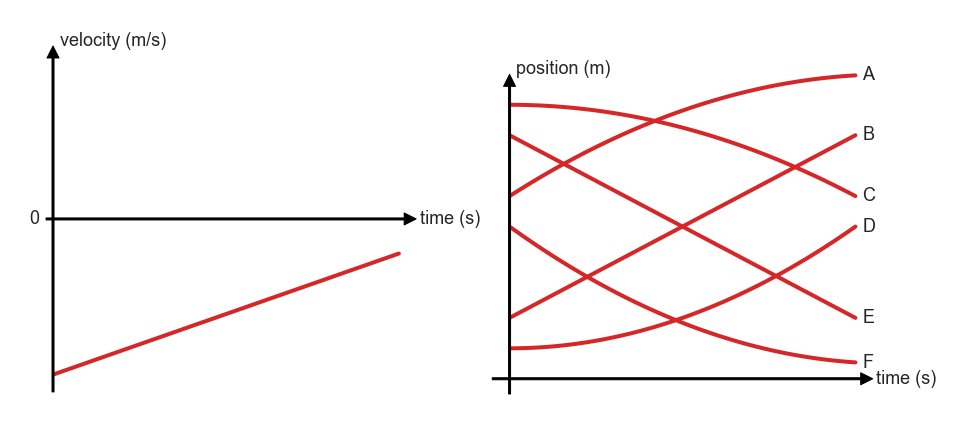
\includegraphics[keepaspectratio]{archive/gifs/match_x_v_009.png}}

\textbf{Exercise 10}
\pandocbounded{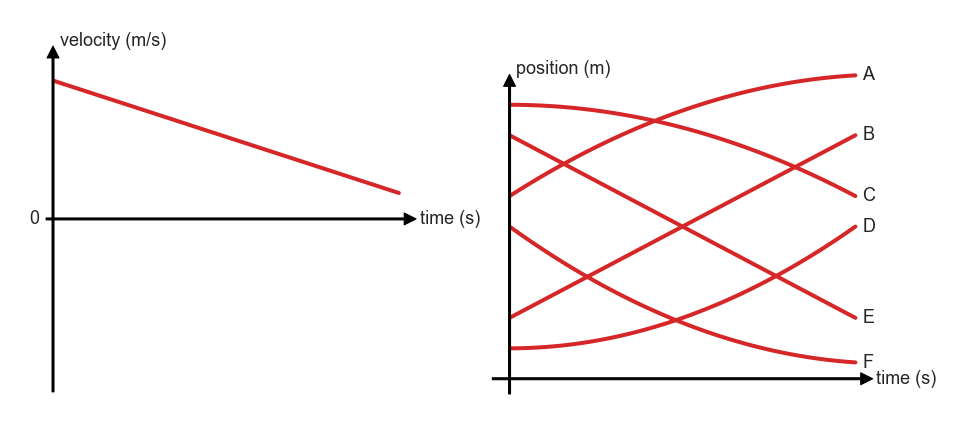
\includegraphics[keepaspectratio]{archive/gifs/match_x_v_010.png}}

\textbf{Exercise 11}
\pandocbounded{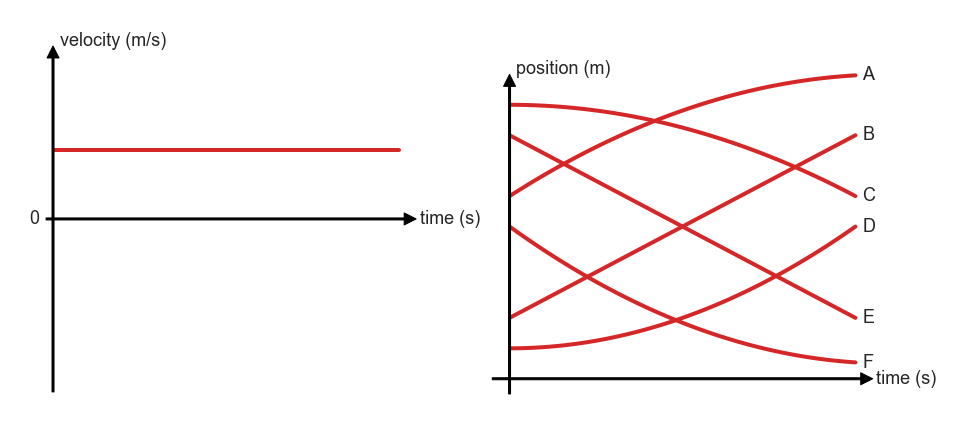
\includegraphics[keepaspectratio]{archive/gifs/match_x_v_011.png}}

\textbf{Exercise 12}
\pandocbounded{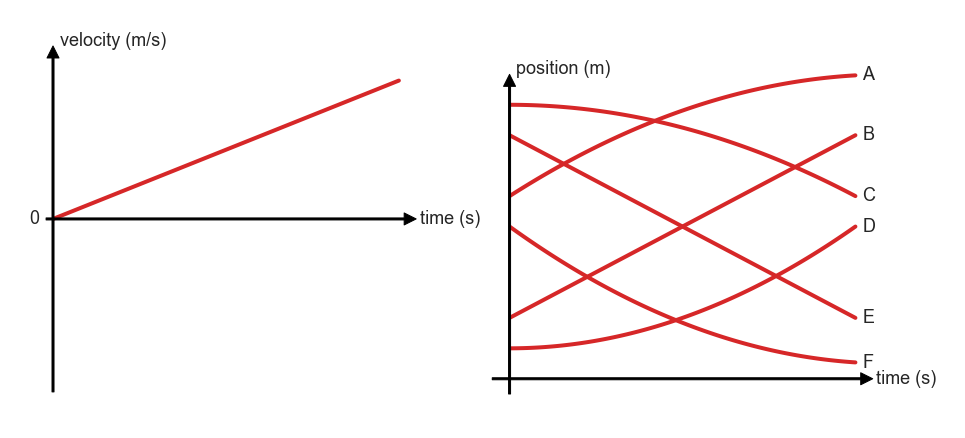
\includegraphics[keepaspectratio]{archive/gifs/match_x_v_012.png}}

\section*{Oil drop patterns}\label{oil-drop-patterns}
\addcontentsline{toc}{section}{Oil drop patterns}

\markright{Oil drop patterns}

Oil drips from a car \emph{at fixed time intervals}. Match the oil drop
pattern the car leaves on the road with the curves on the right.
Attention: there might be more than one solution!

\textbf{Exercise 1}
\pandocbounded{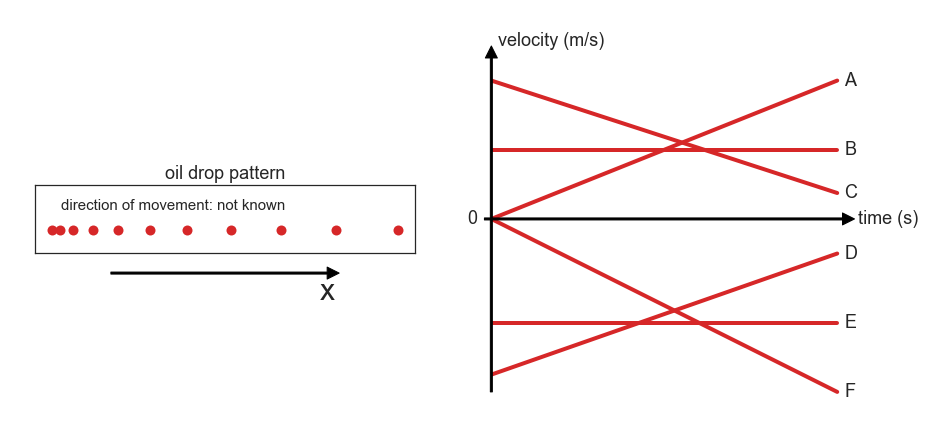
\includegraphics[keepaspectratio]{archive/gifs/match_drop_001.png}}

\textbf{Exercise 2}
\pandocbounded{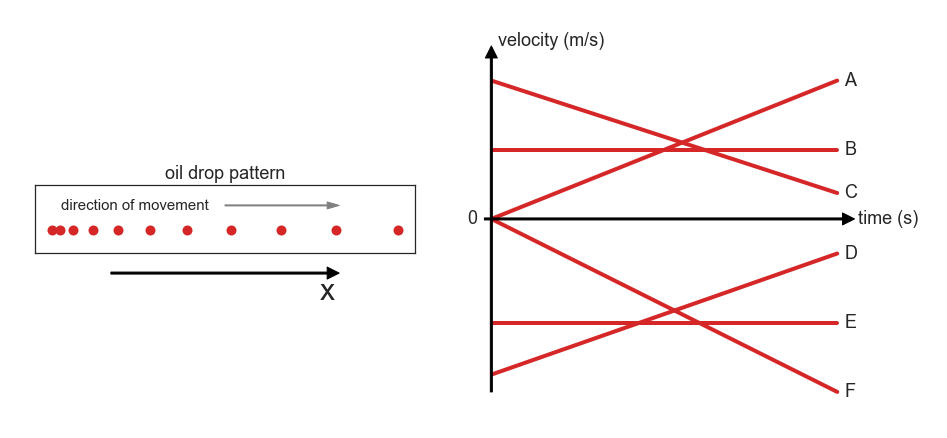
\includegraphics[keepaspectratio]{archive/gifs/match_drop_002.png}}

\textbf{Exercise 3}
\pandocbounded{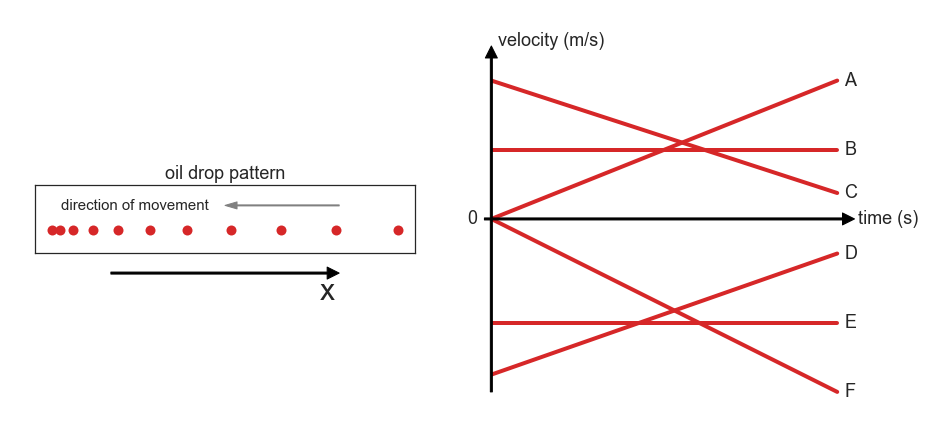
\includegraphics[keepaspectratio]{archive/gifs/match_drop_003.png}}

\textbf{Exercise 4}
\pandocbounded{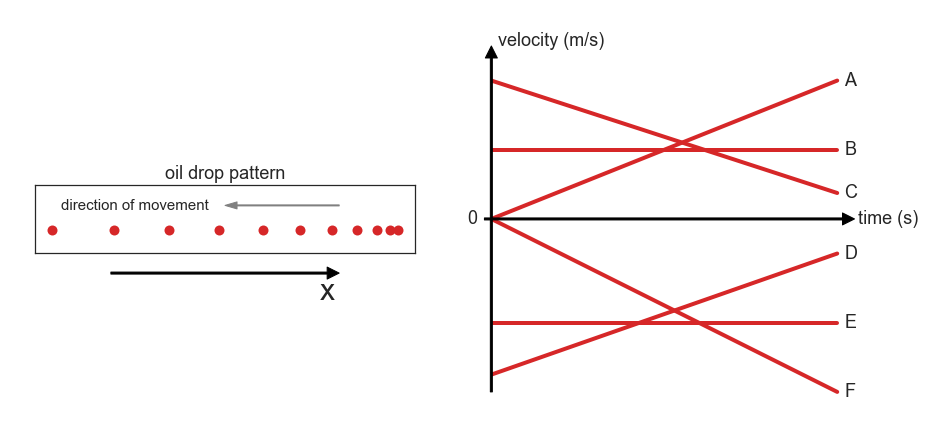
\includegraphics[keepaspectratio]{archive/gifs/match_drop_004.png}}

\textbf{Exercise 5}
\pandocbounded{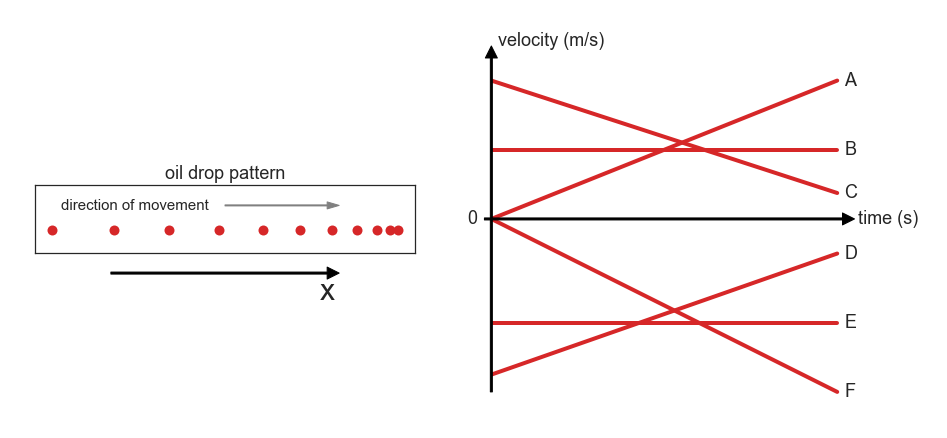
\includegraphics[keepaspectratio]{archive/gifs/match_drop_005.png}}

\textbf{Exercise 6}
\pandocbounded{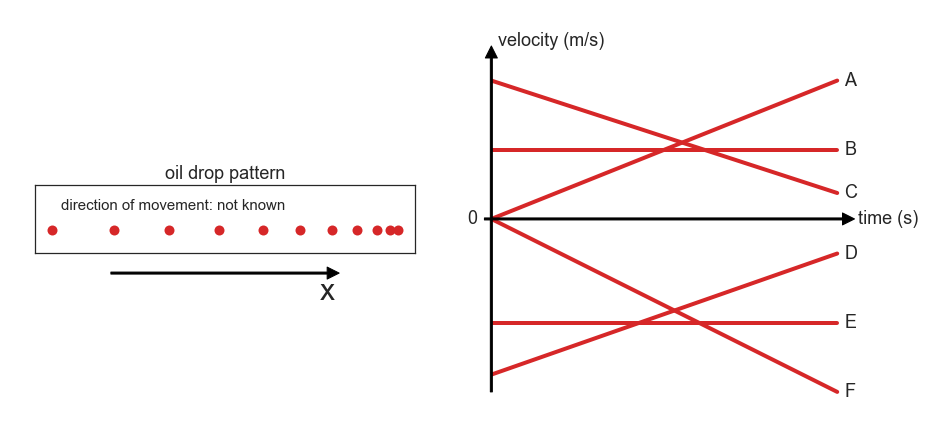
\includegraphics[keepaspectratio]{archive/gifs/match_drop_006.png}}

\textbf{Exercise 7}
\pandocbounded{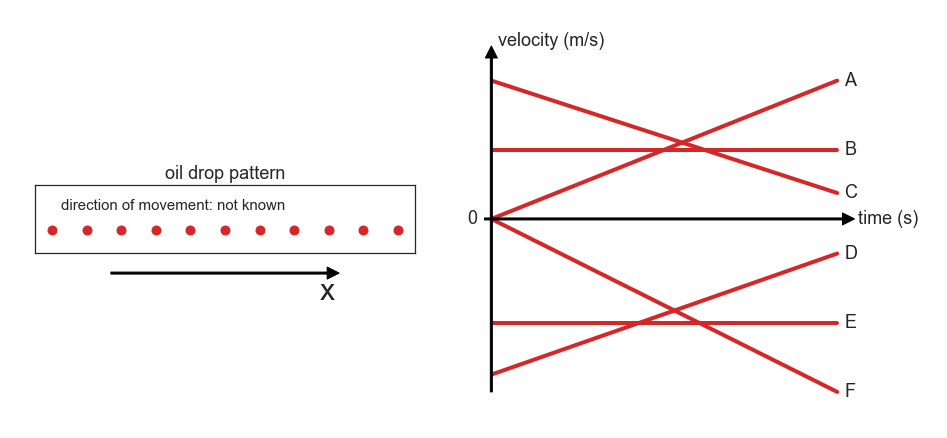
\includegraphics[keepaspectratio]{archive/gifs/match_drop_007.png}}

\textbf{Exercise 8}
\pandocbounded{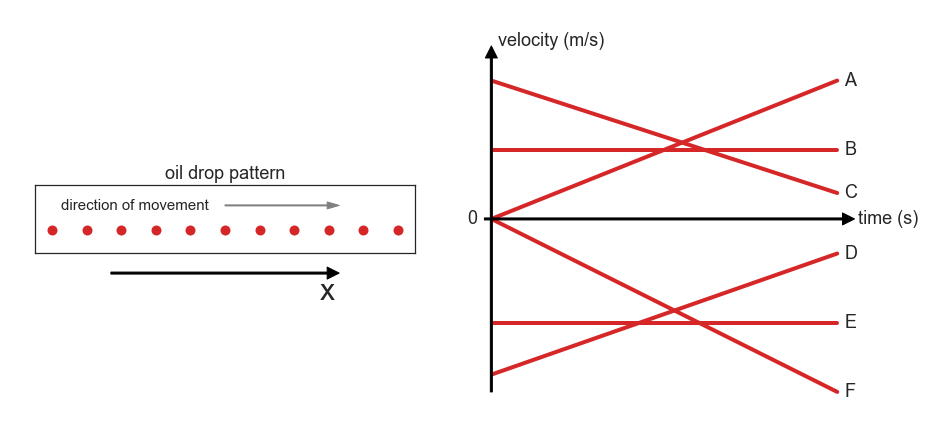
\includegraphics[keepaspectratio]{archive/gifs/match_drop_008.png}}

\textbf{Exercise 9}
\pandocbounded{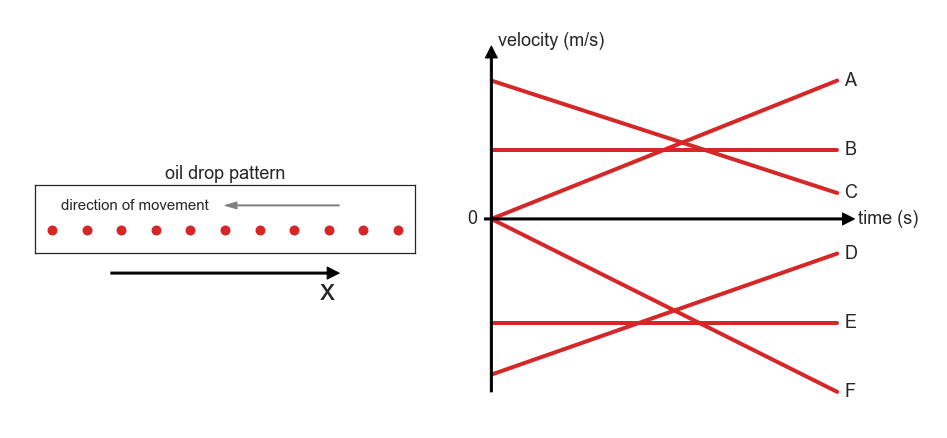
\includegraphics[keepaspectratio]{archive/gifs/match_drop_009.png}}

\textbf{Exercise 10}
\pandocbounded{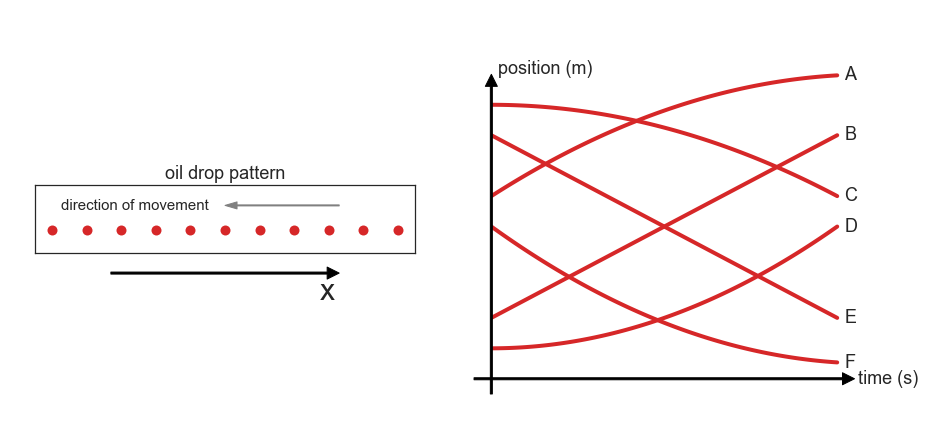
\includegraphics[keepaspectratio]{archive/gifs/match_drop_010.png}}

\textbf{Exercise 11}
\pandocbounded{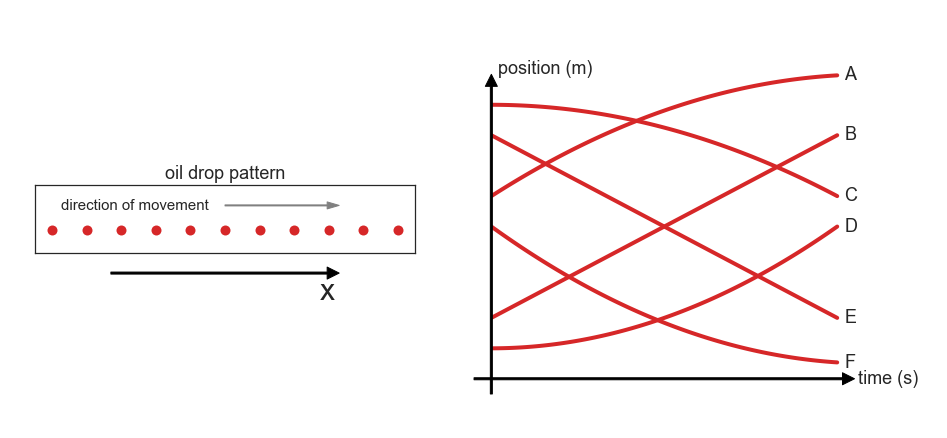
\includegraphics[keepaspectratio]{archive/gifs/match_drop_011.png}}

\textbf{Exercise 12}
\pandocbounded{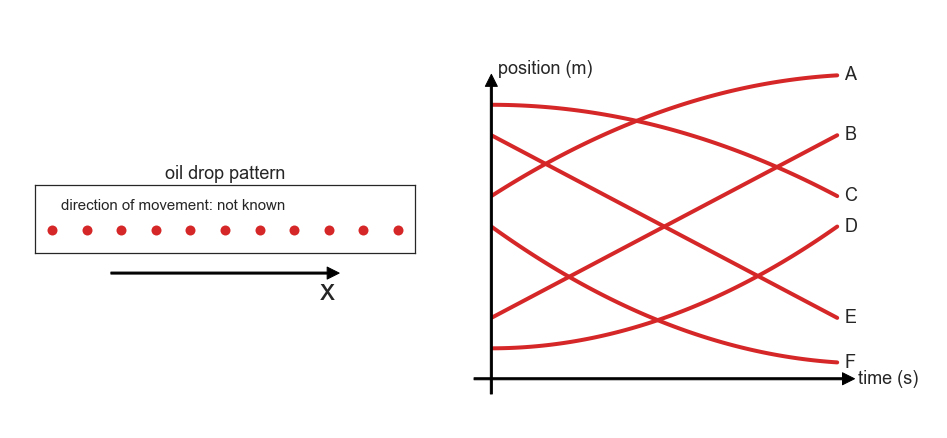
\includegraphics[keepaspectratio]{archive/gifs/match_drop_012.png}}

\textbf{Exercise 13}
\pandocbounded{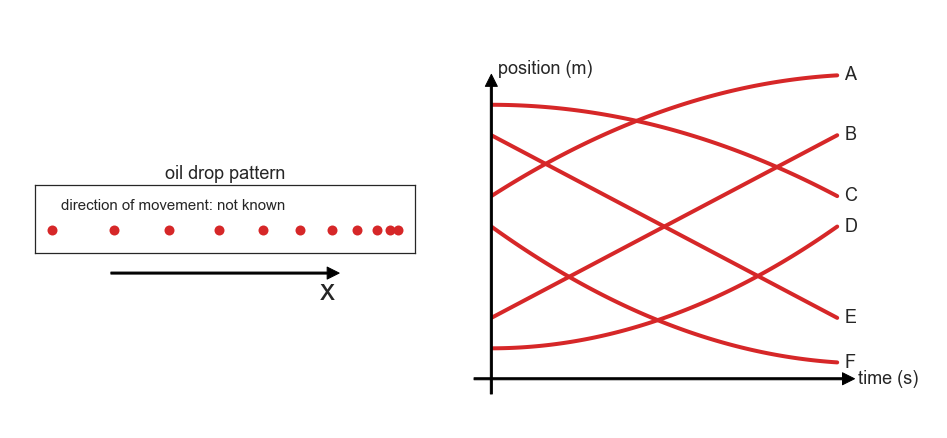
\includegraphics[keepaspectratio]{archive/gifs/match_drop_013.png}}

\textbf{Exercise 14}
\pandocbounded{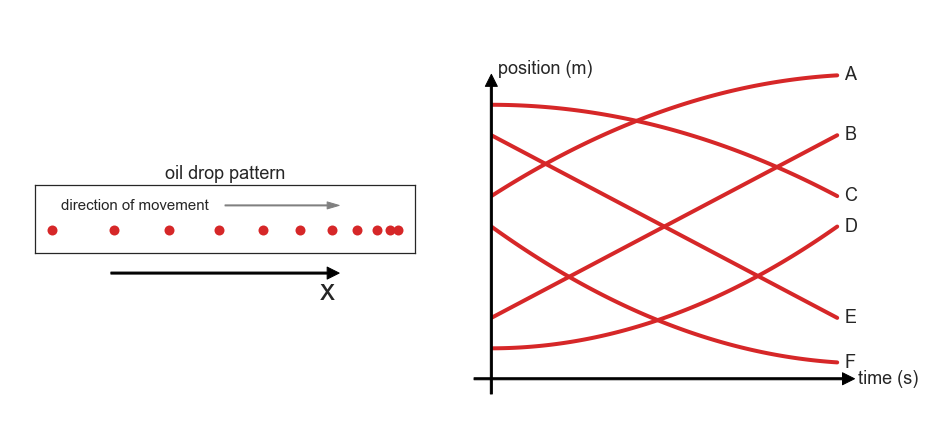
\includegraphics[keepaspectratio]{archive/gifs/match_drop_014.png}}

\textbf{Exercise 15}
\pandocbounded{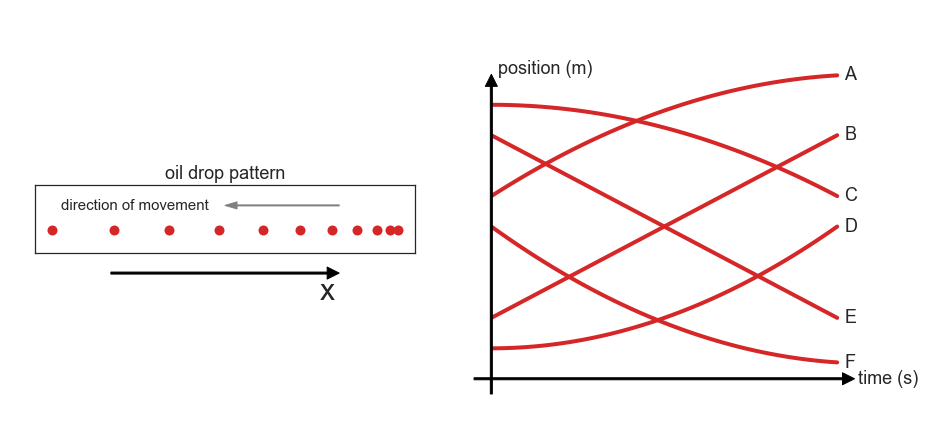
\includegraphics[keepaspectratio]{archive/gifs/match_drop_015.png}}

\textbf{Exercise 16}
\pandocbounded{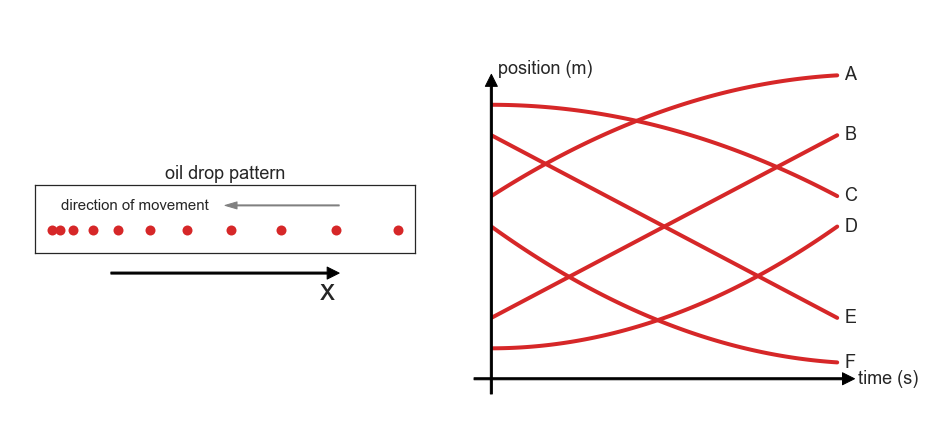
\includegraphics[keepaspectratio]{archive/gifs/match_drop_016.png}}

\textbf{Exercise 17}
\pandocbounded{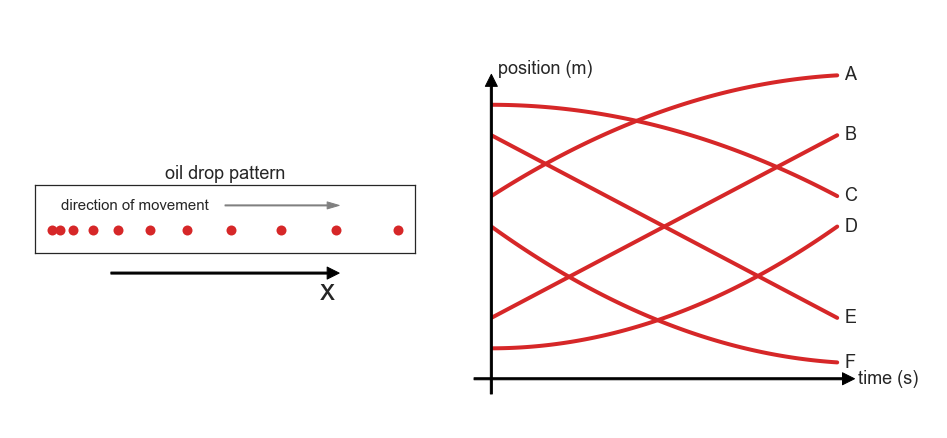
\includegraphics[keepaspectratio]{archive/gifs/match_drop_017.png}}

\textbf{Exercise 18}
\pandocbounded{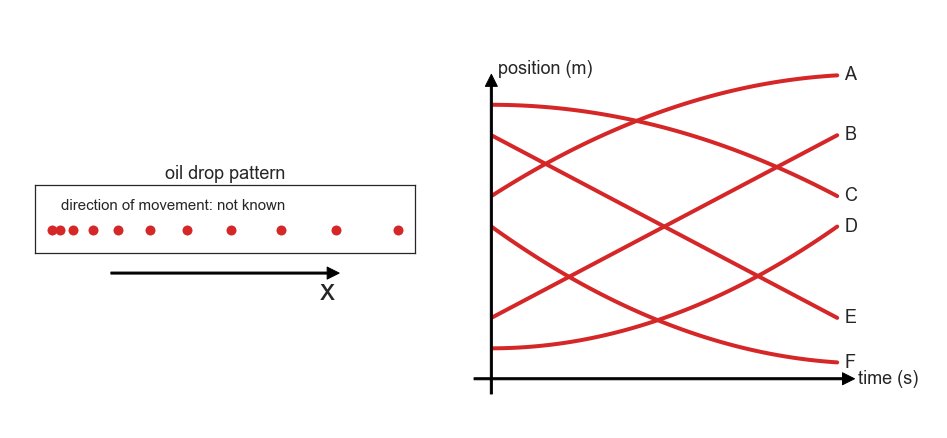
\includegraphics[keepaspectratio]{archive/gifs/match_drop_018.png}}

\chapter*{extra: momentum}\label{extra-momentum}
\addcontentsline{toc}{chapter}{extra: momentum}

\markboth{extra: momentum}{extra: momentum}

\section*{Momentum, Lecture 1}\label{momentum-lecture-1}
\addcontentsline{toc}{section}{Momentum, Lecture 1}

\markright{Momentum, Lecture 1}

\section*{Momentum, Lecture 2}\label{momentum-lecture-2}
\addcontentsline{toc}{section}{Momentum, Lecture 2}

\markright{Momentum, Lecture 2}

Videos of people flying backwards after being shot: *
\href{https://youtu.be/00oG5gtD0Ho}{Bruce Willis} (watch the few first
seconds) * \href{https://youtu.be/BBoP2l7VBeo}{Uma Thurman} *
\href{https://youtu.be/iH9hjyoAugw}{Morgan Freeman} (watch from 1:10)

\section*{Momentum, Lecture 3}\label{momentum-lecture-3}
\addcontentsline{toc}{section}{Momentum, Lecture 3}

\markright{Momentum, Lecture 3}

Videos of a Newton's Cradle *
\href{https://youtu.be/7qPvmYbfM6I}{Newton's Cradle with a High-Speed
Video Camera} * \href{https://youtu.be/8dgyPRA86K0}{Amazing
Demonstration Of A Giant Newton's Cradle!}

\part{the good stuff}

\chapter*{cartoons}\label{cartoons}
\addcontentsline{toc}{chapter}{cartoons}

\markboth{cartoons}{cartoons}

\url{https://www.gocomics.com/calvinandhobbes/2015/01/12}
\pandocbounded{\includegraphics[keepaspectratio]{index_files/mediabag/me593ygilrh01.jpg}}

\url{https://xkcd.com/2207/}
\pandocbounded{\includegraphics[keepaspectratio]{index_files/mediabag/math_work.png}}

\url{https://www.smbc-comics.com/comic/2013-06-16}
\pandocbounded{\includegraphics[keepaspectratio]{index_files/mediabag/20130616.png}}

\href{https://hivemill.com/products/science-abridged-beyond-the-point-of-usefulness}{Science:
Abridged Beyond the Point of Usefulness}
\pandocbounded{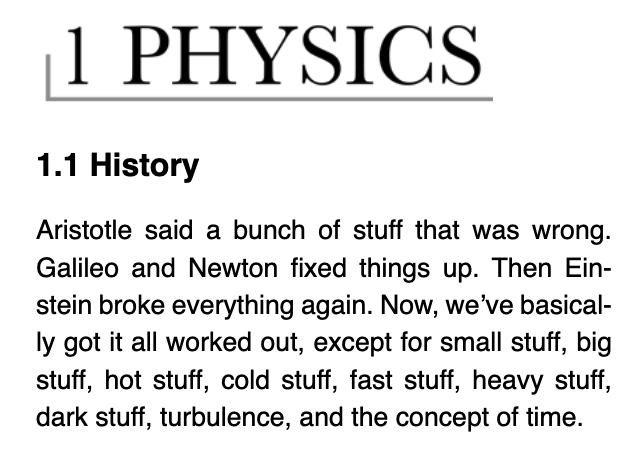
\includegraphics[keepaspectratio]{archive/gifs/Weinersmith-physics-abridged.png}}

\url{http://www.sciencecartoonsplus.com/gallery/physics/galphys2j.php\#}
\pandocbounded{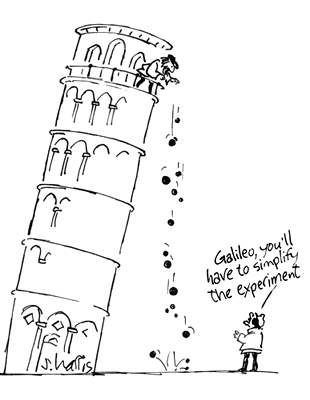
\includegraphics[keepaspectratio]{archive/gifs/physics117_galileo-youll-have-to-simplify.png}}

\pandocbounded{\includegraphics[keepaspectratio]{index_files/mediabag/aqjZq2M_460s.jpg}}

\chapter*{units}\label{units}
\addcontentsline{toc}{chapter}{units}

\markboth{units}{units}

Any time you pick up a well shuffled deck, you are almost certainly
holding an arrangement of cards that has never before existed and will
likely never exist again. \(52! \approx 10^{68}\). Suppose a new
permutation of 52 cards was drawn every second starting from The Big
Bang (13.8 billion years ago). You wouldn't even be close. To count out
all 52! permutations you would need \(10^{51}\) ages of the universe.
\pandocbounded{\includegraphics[keepaspectratio]{index_files/mediabag/1-6NrFpflyvQ3WzklkfB.jpg}}

Any time you pick up a well shuffled deck, you are almost certainly
holding an arrangement of cards that has never before existed and will
likely never exist again. - Yannay Khaikin pic.twitter.com/afOpu0y7qA

--- 〈 Berger \textbar{} Dillon 〉 (@InertialObservr) September 18, 2019

If you worked every single day, making \$5000/day, from the time
Columbus sailed to America, to the time you are reading this tweet, you
would still not be a billionaire.

How much larger/heavier/longer was the Megalodon compared with a great
white?
\pandocbounded{\includegraphics[keepaspectratio]{index_files/mediabag/I5C92rHZpx1uyhe2DLxq.jpg}}

This is the mass damper of the Taipei 101 skyscraper: it has a mass of
728 tons and a diameter of 5.4 meters. It helps stabilize the building
in high winds and this is the record movement realized during typhoon
Soudelor with 160 km/h winds \textbf{what is the mass density of this
ball?}\\

This is the mass damper of the Taipei 101 skyscraper: it has a mass of
728 tons and a diameter of 5.4 meters. It helps stabilize the building
in high winds and this is the record movement realized during typhoon
Soudelor with 160 km/h winds https://t.co/e0MxA0iOG5
pic.twitter.com/xqcbyUNJWs

--- Massimo (@Rainmaker1973) September 8, 2018

\begin{quote}
https://www.youtube.com/watch?v=xqELmBNyWfU
\end{quote}

orders of magnitude, from

\begin{quote}
https://twitter.com/Rainmaker1973/status/1125710475378012161
\end{quote}

\pandocbounded{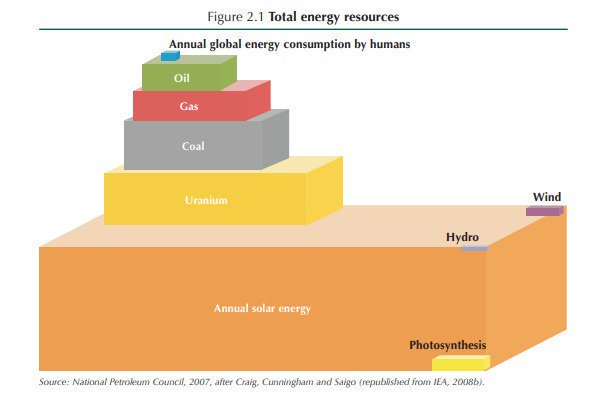
\includegraphics[keepaspectratio]{archive/gifs/energy-orders-of-magnitude.jpg}}

\pandocbounded{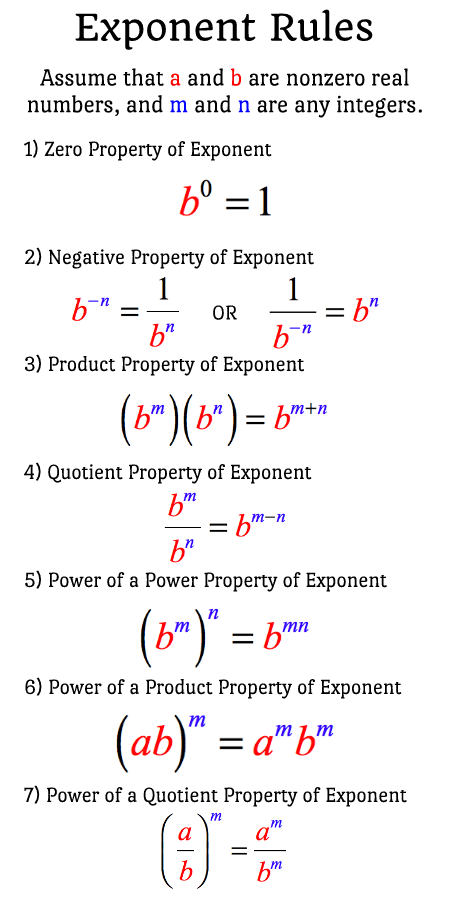
\includegraphics[keepaspectratio]{archive/gifs/exponents.png}}

\chapter*{kinematics}\label{kinematics}
\addcontentsline{toc}{chapter}{kinematics}

\markboth{kinematics}{kinematics}

\section*{Motivation for studying
kinematics}\label{motivation-for-studying-kinematics}
\addcontentsline{toc}{section}{Motivation for studying kinematics}

\markright{Motivation for studying kinematics}

\href{https://youtu.be/aFzyqFrUUFc?t=105}{firefighting airplanes in
action},
\href{https://giphy.com/gifs/cute-aww-eyebleach-OOTtmh8oXrFK5ccNU7}{dogs
jumping into a car},
\href{https://www.youtube.com/watch?v=LcCA5z-I_iU}{woman walking the
wrong way}

\section*{X and Y movements are
independent}\label{x-and-y-movements-are-independent}
\addcontentsline{toc}{section}{X and Y movements are independent}

\markright{X and Y movements are independent}

\#PhysicsFactlet (179)The rate of change of position is velocity.The
rate of change of velocity is acceleration.The rate of change of
acceleration is jerk.The rate of change of jerk is jounce.The rate of
change of jounce is crackle.The rate of change of crackle is pop.

--- Jacopo Bertolotti (@j\_bertolotti) October 8, 2019

\section*{2d kinematics}\label{d-kinematics}
\addcontentsline{toc}{section}{2d kinematics}

\markright{2d kinematics}

\subsection*{Harlem Globetrotter Makes Incredible Trick Shot From Plane
Flying 70
MPH}\label{harlem-globetrotter-makes-incredible-trick-shot-from-plane-flying-70-mph}
\addcontentsline{toc}{subsection}{Harlem Globetrotter Makes Incredible
Trick Shot From Plane Flying 70 MPH}

\subsection*{jumping goats}\label{jumping-goats}
\addcontentsline{toc}{subsection}{jumping goats}

\subsection*{Kevin failed Physics}\label{kevin-failed-physics}
\addcontentsline{toc}{subsection}{Kevin failed Physics}

Yes, Kevin failed physics and math, but he knew how to build a helluva
ramp! 🍺 🥴 pic.twitter.com/8rPrtRmCYy

--- 🍺 Hold My Beer 🍺 (@HldMyBeer) August 31, 2021

\section*{Galilean relativity}\label{galilean-relativity}
\addcontentsline{toc}{section}{Galilean relativity}

\markright{Galilean relativity}

\subsection*{swimming against the
current}\label{swimming-against-the-current}
\addcontentsline{toc}{subsection}{swimming against the current}

\subsection*{Mythbusters - Soccer Ball Shot from
Truck}\label{mythbusters---soccer-ball-shot-from-truck}
\addcontentsline{toc}{subsection}{Mythbusters - Soccer Ball Shot from
Truck}

https://youtu.be/BLuI118nhzc

\section*{Circular motion}\label{circular-motion}
\addcontentsline{toc}{section}{Circular motion}

\markright{Circular motion}

\subsection*{Hamster, from
https://twitter.com/SJSchauer/status/1186484325451227136?s=09}\label{hamster-from-httpstwitter.comsjschauerstatus1186484325451227136s09}
\addcontentsline{toc}{subsection}{Hamster, from
https://twitter.com/SJSchauer/status/1186484325451227136?s=09}

\subsection*{Human Loop the Loop with Damien
Walters}\label{human-loop-the-loop-with-damien-walters}
\addcontentsline{toc}{subsection}{Human Loop the Loop with Damien
Walters}

\subsection*{Ball in a pie pan: Testing
Experiment}\label{ball-in-a-pie-pan-testing-experiment}
\addcontentsline{toc}{subsection}{Ball in a pie pan: Testing Experiment}

\subsection*{Beer flipping}\label{beer-flipping}
\addcontentsline{toc}{subsection}{Beer flipping}

\subsection*{2001: A Space Odyssey}\label{a-space-odyssey}
\addcontentsline{toc}{subsection}{2001: A Space Odyssey}

\subsection*{Centripetal force}\label{centripetal-force}
\addcontentsline{toc}{subsection}{Centripetal force}

Many forces can take the role of the centripetal force.

\pandocbounded{\includegraphics[keepaspectratio]{archive/gifs/centripetal-force.png}}

\chapter*{Newton's laws}\label{newtons-laws}
\addcontentsline{toc}{chapter}{Newton's laws}

\markboth{Newton's laws}{Newton's laws}

\section*{Newton's first law}\label{newtons-first-law}
\addcontentsline{toc}{section}{Newton's first law}

\markright{Newton's first law}

\subsection*{The fall of the dinosaurs}\label{the-fall-of-the-dinosaurs}
\addcontentsline{toc}{subsection}{The fall of the dinosaurs}

\subsection*{Trampoline with leaves}\label{trampoline-with-leaves}
\addcontentsline{toc}{subsection}{Trampoline with leaves}

\subsection*{At the Kibo ISS module}\label{at-the-kibo-iss-module}
\addcontentsline{toc}{subsection}{At the Kibo ISS module}

\subsection*{\texorpdfstring{\href{https://youtu.be/wUeSW0rUkao?t=174}{Rollerblades
on a moving
table}}{Rollerblades on a moving table}}\label{rollerblades-on-a-moving-table}
\addcontentsline{toc}{subsection}{\href{https://youtu.be/wUeSW0rUkao?t=174}{Rollerblades
on a moving table}}

\subsection*{What is Inertia?}\label{what-is-inertia}
\addcontentsline{toc}{subsection}{What is Inertia?}

\pandocbounded{\includegraphics[keepaspectratio]{archive/gifs/inertia.jpg}}

\section*{Newton's second law}\label{newtons-second-law}
\addcontentsline{toc}{section}{Newton's second law}

\markright{Newton's second law}

\subsection*{Man with superhuman
strength}\label{man-with-superhuman-strength}
\addcontentsline{toc}{subsection}{Man with superhuman strength}

\subsection*{Inside the ISS}\label{inside-the-iss}
\addcontentsline{toc}{subsection}{Inside the ISS}

\subsection*{Whack-a-Stack}\label{whack-a-stack}
\addcontentsline{toc}{subsection}{Whack-a-Stack}

\subsection*{Apollo 15 hammer-feather
drop}\label{apollo-15-hammer-feather-drop}
\addcontentsline{toc}{subsection}{Apollo 15 hammer-feather drop}

\section*{Newton's third law}\label{newtons-third-law}
\addcontentsline{toc}{section}{Newton's third law}

\markright{Newton's third law}

\subsection*{Newton cartoon}\label{newton-cartoon}
\addcontentsline{toc}{subsection}{Newton cartoon}

\pandocbounded{\includegraphics[keepaspectratio]{archive/gifs/newton-slaps-car.jpg}}

\subsection*{Motorcycle kicks car}\label{motorcycle-kicks-car}
\addcontentsline{toc}{subsection}{Motorcycle kicks car}

\section*{Friction}\label{friction}
\addcontentsline{toc}{section}{Friction}

\markright{Friction}

\subsection*{Static friction}\label{static-friction}
\addcontentsline{toc}{subsection}{Static friction}

\subsection*{Static vs.~kinetic
friction}\label{static-vs.-kinetic-friction}
\addcontentsline{toc}{subsection}{Static vs.~kinetic friction}

\subsection*{No friction on inclined
plane}\label{no-friction-on-inclined-plane}
\addcontentsline{toc}{subsection}{No friction on inclined plane}

\subsection*{Cat fails to jump, not enough
friction}\label{cat-fails-to-jump-not-enough-friction}
\addcontentsline{toc}{subsection}{Cat fails to jump, not enough
friction}

\subsection*{Spidergirl}\label{spidergirl}
\addcontentsline{toc}{subsection}{Spidergirl}

\chapter*{linear momentum \& center of
mass}\label{linear-momentum-center-of-mass}
\addcontentsline{toc}{chapter}{linear momentum \& center of mass}

\markboth{linear momentum \& center of mass}{linear momentum \& center
of mass}

\section*{Collisions}\label{collisions}
\addcontentsline{toc}{section}{Collisions}

\markright{Collisions}

\subsection*{brain during collision}\label{brain-during-collision}
\addcontentsline{toc}{subsection}{brain during collision}

\subsection*{golf ball}\label{golf-ball}
\addcontentsline{toc}{subsection}{golf ball}

\subsection*{Football to the Face 1000x Slower - The Slow Mo
Guys}\label{football-to-the-face-1000x-slower---the-slow-mo-guys}
\addcontentsline{toc}{subsection}{Football to the Face 1000x Slower -
The Slow Mo Guys}

\section*{Elastic collisions}\label{elastic-collisions}
\addcontentsline{toc}{section}{Elastic collisions}

\markright{Elastic collisions}

\subsection*{failed collision}\label{failed-collision}
\addcontentsline{toc}{subsection}{failed collision}

\subsection*{bullets ricochet off
water}\label{bullets-ricochet-off-water}
\addcontentsline{toc}{subsection}{bullets ricochet off water}

\subsection*{periodic billiard
collision}\label{periodic-billiard-collision}
\addcontentsline{toc}{subsection}{periodic billiard collision}

\subsection*{Althea Reinhardt's face
save}\label{althea-reinhardts-face-save}
\addcontentsline{toc}{subsection}{Althea Reinhardt's face save}

\{\% twitter
https://twitter.com/BeardedGenius/status/1472221793595310084 \%\}\\
\pandocbounded{\includegraphics[keepaspectratio]{index_files/mediabag/FG5giisXsAI-U6a-form.pdf}}

\section*{Inelastic collisions}\label{inelastic-collisions}
\addcontentsline{toc}{section}{Inelastic collisions}

\markright{Inelastic collisions}

\subsection*{Apple collision at 90
km/h.}\label{apple-collision-at-90-kmh.}
\addcontentsline{toc}{subsection}{Apple collision at 90 km/h.}

\section*{Center of mass}\label{center-of-mass}
\addcontentsline{toc}{section}{Center of mass}

\markright{Center of mass}

\subsection*{center of mass parabolic
trajectory}\label{center-of-mass-parabolic-trajectory}
\addcontentsline{toc}{subsection}{center of mass parabolic trajectory}

\subsection*{Josh Imatorbhebhe vertical
jump}\label{josh-imatorbhebhe-vertical-jump}
\addcontentsline{toc}{subsection}{Josh Imatorbhebhe vertical jump}

\section*{Internal vs external
forces}\label{internal-vs-external-forces}
\addcontentsline{toc}{section}{Internal vs external forces}

\markright{Internal vs external forces}

\subsection*{How to push your pickup
truck}\label{how-to-push-your-pickup-truck}
\addcontentsline{toc}{subsection}{How to push your pickup truck}

\chapter*{energy}\label{energy}
\addcontentsline{toc}{chapter}{energy}

\markboth{energy}{energy}

\section*{Elastic energy}\label{elastic-energy}
\addcontentsline{toc}{section}{Elastic energy}

\markright{Elastic energy}

\subsection*{The First Hold \& Release Bungee Jump \textbar{} Damien
Walters}\label{the-first-hold-release-bungee-jump-damien-walters}
\addcontentsline{toc}{subsection}{The First Hold \& Release Bungee Jump
\textbar{} Damien Walters}

https://youtu.be/iN1beukMJJc

\section*{Potential and Kinetic
Energy}\label{potential-and-kinetic-energy}
\addcontentsline{toc}{section}{Potential and Kinetic Energy}

\markright{Potential and Kinetic Energy}

\subsection*{Visualization of conservation of
energy}\label{visualization-of-conservation-of-energy}
\addcontentsline{toc}{subsection}{Visualization of conservation of
energy}

\subsection*{High road low road track race, potential-kinetic energy
tracks}\label{high-road-low-road-track-race-potential-kinetic-energy-tracks}
\addcontentsline{toc}{subsection}{High road low road track race,
potential-kinetic energy tracks}

\url{https://youtu.be/_GJujClGYJQ}

\subsection*{Mondo Duplantis 2018, play at 0.25
speed}\label{mondo-duplantis-2018-play-at-0.25-speed}
\addcontentsline{toc}{subsection}{Mondo Duplantis 2018, play at 0.25
speed}

\subsection*{150 Ton Hydraulic Guillotine Vs Deck of
Cards}\label{ton-hydraulic-guillotine-vs-deck-of-cards}
\addcontentsline{toc}{subsection}{150 Ton Hydraulic Guillotine Vs Deck
of Cards}

\chapter*{fluids}\label{fluids}
\addcontentsline{toc}{chapter}{fluids}

\markboth{fluids}{fluids}

How a 50 kg iron working anvil floats on liquid mercury From
https://twitter.com/Rainmaker1973/status/1194215829199605765?s=09

\section*{Hydrostatic pressure}\label{hydrostatic-pressure}
\addcontentsline{toc}{section}{Hydrostatic pressure}

\markright{Hydrostatic pressure}

\subsection*{Pressure change during
diving}\label{pressure-change-during-diving}
\addcontentsline{toc}{subsection}{Pressure change during diving}

\{\% twitter
https://twitter.com/physicsastronmy/status/1464007031367602181?s=12 \%\}

\subsection*{Fish tower}\label{fish-tower}
\addcontentsline{toc}{subsection}{Fish tower}

\subsection*{The Hydrostatic Paradox -
Explained!}\label{the-hydrostatic-paradox---explained}
\addcontentsline{toc}{subsection}{The Hydrostatic Paradox - Explained!}

\subsection*{Pascal's Blaising Barrel - Exploding Glass Barrel with
Water
Pressure}\label{pascals-blaising-barrel---exploding-glass-barrel-with-water-pressure}
\addcontentsline{toc}{subsection}{Pascal's Blaising Barrel - Exploding
Glass Barrel with Water Pressure}

\subsection*{The Pressure Paradox \#VeritasiumContest
\#GrandPrizeWinner}\label{the-pressure-paradox-veritasiumcontest-grandprizewinner}
\addcontentsline{toc}{subsection}{The Pressure Paradox
\#VeritasiumContest \#GrandPrizeWinner}

\section*{Surface tension}\label{surface-tension}
\addcontentsline{toc}{section}{Surface tension}

\markright{Surface tension}

from https://twitter.com/Rainmaker1973/status/1191329332926570497?s=09

\chapter*{wow}\label{wow}
\addcontentsline{toc}{chapter}{wow}

\markboth{wow}{wow}

\subsection*{rope swing record}\label{rope-swing-record}
\addcontentsline{toc}{subsection}{rope swing record}

does the period of a pendulum depend on its mass?

\subsection*{Time-Lapse: Lose Yourself in the Night
Sky}\label{time-lapse-lose-yourself-in-the-night-sky}
\addcontentsline{toc}{subsection}{Time-Lapse: Lose Yourself in the Night
Sky}

\subsection*{fastest response time}\label{fastest-response-time}
\addcontentsline{toc}{subsection}{fastest response time}

The kangaroo rat's escape response to a snake attack is less than 70
milliseconds and the quickest mammalian startle response.

\subsection*{Selected solar system objects to scale in size, rotation
speed and axial
tilt}\label{selected-solar-system-objects-to-scale-in-size-rotation-speed-and-axial-tilt}
\addcontentsline{toc}{subsection}{Selected solar system objects to scale
in size, rotation speed and axial tilt}

\subsection*{Milky Way and Earth}\label{milky-way-and-earth}
\addcontentsline{toc}{subsection}{Milky Way and Earth}

Milky Way spinning around Earth

Milky Way fixed, earth spinning round

\subsection*{The Milky Way Fly Out}\label{the-milky-way-fly-out}
\addcontentsline{toc}{subsection}{The Milky Way Fly Out}

Stefan Payne-Wardenaar

\subsection*{Least action, path of bowling ball minimizes
action}\label{least-action-path-of-bowling-ball-minimizes-action}
\addcontentsline{toc}{subsection}{Least action, path of bowling ball
minimizes action}

\subsection*{A free-falling frame of reference cancels
gravity}\label{a-free-falling-frame-of-reference-cancels-gravity}
\addcontentsline{toc}{subsection}{A free-falling frame of reference
cancels gravity}

\{\% twitter https://twitter.com/sfera314/status/1173284029900173315
\%\}

\subsection*{Mesmerising Mass Sheep
Herding}\label{mesmerising-mass-sheep-herding}
\addcontentsline{toc}{subsection}{Mesmerising Mass Sheep Herding}

\subsection*{Solar eclipse from space}\label{solar-eclipse-from-space}
\addcontentsline{toc}{subsection}{Solar eclipse from space}

\subsection*{150 Ton Hydraulic Guillotine Vs Deck of
Cards}\label{ton-hydraulic-guillotine-vs-deck-of-cards-1}
\addcontentsline{toc}{subsection}{150 Ton Hydraulic Guillotine Vs Deck
of Cards}

\bookmarksetup{startatroot}

\chapter*{exams}\label{exams}
\addcontentsline{toc}{chapter}{exams}

\markboth{exams}{exams}

Some past exams (in hebrew):

\begin{longtable}[]{@{}
  >{\centering\arraybackslash}p{(\linewidth - 8\tabcolsep) * \real{0.2000}}
  >{\centering\arraybackslash}p{(\linewidth - 8\tabcolsep) * \real{0.2000}}
  >{\centering\arraybackslash}p{(\linewidth - 8\tabcolsep) * \real{0.2000}}
  >{\centering\arraybackslash}p{(\linewidth - 8\tabcolsep) * \real{0.2000}}
  >{\centering\arraybackslash}p{(\linewidth - 8\tabcolsep) * \real{0.2000}}@{}}
\toprule\noalign{}
\begin{minipage}[b]{\linewidth}\centering
Year
\end{minipage} & \begin{minipage}[b]{\linewidth}\centering
Midterm
\end{minipage} & \begin{minipage}[b]{\linewidth}\centering
Moed A
\end{minipage} & \begin{minipage}[b]{\linewidth}\centering
Moed B
\end{minipage} & \begin{minipage}[b]{\linewidth}\centering
Moed C
\end{minipage} \\
\midrule\noalign{}
\endhead
\bottomrule\noalign{}
\endlastfoot
2021-2022 & \href{./archive/exams/2022-71031-bochan.pdf}{}  
\href{./archive/exams/2022-71031-bochan-solution.pdf}{} &
\href{./archive/exams/2022-71031-moed-A.pdf}{}  
\href{./archive/exams/2022-71031-moed-A-solution.pdf}{} &
\href{./archive/exams/2022-71031-moed-B.pdf}{}  
\href{./archive/exams/2022-71031-moed-B-solution.pdf}{} & \\
2020-2021 & \href{./archive/exams/2021-71031-bochan.pdf}{}  
\href{./archive/exams/2021-71031-bochan-solution.pdf}{} &
\href{./archive/exams/2021-71031-moed-A.pdf}{}  
\href{./archive/exams/2021-71031-moed-A-solution.pdf}{} &
\href{./archive/exams/2021-71031-moed-B.pdf}{}  
\href{./archive/exams/2021-71031-moed-B-solution.pdf}{} & \\
2019-2020 & \href{./archive/exams/2020-71031-bochan.pdf}{}  
\href{./archive/exams/2020-71031-bochan-solution.pdf}{} &
\href{./archive/exams/2020-71031-moed-A.pdf}{}  
\href{./archive/exams/2020-71031-moed-A-solution.pdf}{} &
\href{./archive/exams/2020-71031-moed-B.pdf}{}  
\href{./archive/exams/2020-71031-moed-B-solution.pdf}{} &
\href{./archive/exams/2020-71031-moed-C.pdf}{}  
\href{./archive/exams/2020-71031-moed-C-solution.pdf}{} \\
2018-2019 & \href{./archive/exams/2019-71031-bochan.pdf}{}  
\href{./archive/exams/2019-71031-bochan-solution.pdf}{} &
\href{./archive/exams/2019-71031-moed-A.pdf}{}  
\href{./archive/exams/2019-71031-moed-A-solution.pdf}{} &
\href{./archive/exams/2019-71031-moed-B.pdf}{}  
\href{./archive/exams/2019-71031-moed-B-solution.pdf}{} & \\
2017-2018 & \href{./archive/exams/2018-71031-bochan.pdf}{}  
\href{./archive/exams/2018-71031-bochan-solution.pdf}{} &
\href{./archive/exams/2018-71031-moed-A.pdf}{}  
\href{./archive/exams/2018-71031-moed-A-solution.pdf}{} &
\href{./archive/exams/2018-71031-moed-B.pdf}{}  
\href{./archive/exams/2018-71031-moed-B-solution.pdf}{} & \\
\end{longtable}

\bookmarksetup{startatroot}

\chapter*{more stuff}\label{more-stuff}
\addcontentsline{toc}{chapter}{more stuff}

\markboth{more stuff}{more stuff}

\href{./gifs/cartoons.qmd}{Physics cartoons}

Great online Physics resources:

\begin{itemize}
\tightlist
\item
  \href{https://www.khanacademy.org/science/physics}{Khan Academy -
  English}
\item
  \href{http://www.hebrewkhan.org/\#physics}{Khan Academy - עברית}
\item
  \href{https://www.youtube.com/c/MichelvanBiezen/playlists}{Michel van
  Biezen}
\item
  \href{https://www.youtube.com/playlist?list=PLyQSN7X0ro203puVhQsmCj9qhlFQ-As8e}{Walter
  Lewin's 8.01x - MIT Physics I: Classical Mechanics}
\item
  \href{https://phet.colorado.edu/en/simulations/filter?subjects=motion,work-energy-and-power&type=html&sort=alpha&view=grid}{PhET:
  fun, free, interactive, research-based science and mathematics
  simulations}
\end{itemize}




\end{document}
